--- /home/jesse/Analysis/FemtoAnalysis/LamKPublication/CERN/2_EB/LamKPublication_v4.tex
+++ /home/jesse/Analysis/FemtoAnalysis/LamKPublication/CERN/2_EB/LamKPublication_v5.tex
@@ -129,8 +129,8 @@
 %
 
 %%% Put your own title + short title here:
-\title{\LamK femtoscopy in Pb-Pb collisions at $\sqrt{s_{\mathrm{NN}}} = $ 2.76 TeV}
-\ShortTitle{\LamK femtoscopy in Pb-Pb collisions}   % appears on right page headers
+\title{\LamK femtoscopy in Pb--Pb collisions at $\mathbf{\sqrt{{\textit s}_{NN}}} =$ 2.76 TeV}
+\ShortTitle{\LamK femtoscopy in Pb--Pb collisions}   % appears on right page headers
 
 %%% Do not change the next lines
 \Collaboration{ALICE Collaboration\thanks{See Appendix~\ref{app:collab} for the list of collaboration members}}
@@ -139,14 +139,14 @@
 \begin{abstract}
 %%%%%%%%%%%%%%%%%%%%%% Do not use any of the shorthand definitions in the abstract %%%%%%%%%%%%%%%%%%%%%%%%%%%%%%%%%%%
 The first measurements of the scattering parameters of $\Lambda$K pairs in all three charge combinations ($\Lambda$K$^{+}$, $\Lambda$K$^{-}$, and $\Lambda\mathrm{K^{0}_{S}}$) are presented.
-The measurements are achieved through a femtoscopic analysis of $\Lambda$K correlations in Pb-Pb collisions at $\sqrt{s_{\mathrm{NN}}}$ = 2.76 TeV from ALICE at the LHC.  
+The results are achieved through a femtoscopic analysis of $\Lambda$K correlations in Pb--Pb collisions at $\sqrt{s_{\mathrm{NN}}}$ = 2.76 TeV recorded by ALICE at the LHC.  
 The femtoscopic correlations result from strong final-state interactions, and are fit with a parametrization allowing for both the characterization of the pair emission source and the measurement of the scattering parameters for the particle pairs.
 Extensive studies with the THERMINATOR 2 event generator provide a good description of the non-femtoscopic background, which result mainly from collective effects, with unprecedented precision.
 Furthermore, this model together with HIJING simulations are used to account for contributions from residual correlations induced by feed-down from resonances.
 The extracted scattering parameters indicate that the strong force is repulsive in the \LamKchP interaction and attractive in the \LamKchM and \LamKs interactions.
-The results suggest an effect arising from different quark-antiquark interactions between the pairs ($\rm s\overline{s}$ in $\Lambda$K$^{+}$ and $\rm u\overline{u}$ in $\Lambda$K$^{-}$), or from different net strangeness for each system (S=0 for $\Lambda$K$^{+}$, and S=$-2$ for $\Lambda$K$^{-}$).
+The results suggest an effect arising from different quark--antiquark interactions between the pairs ($\rm s\overline{s}$ in $\Lambda$K$^{+}$ and $\rm u\overline{u}$ in $\Lambda$K$^{-}$), or from different net strangeness for each system (S=0 for $\Lambda$K$^{+}$, and S=$-2$ for $\Lambda$K$^{-}$).
 Finally, the $\Lambda$K systems exhibit source radii larger than expected from extrapolation from identical particle femtoscopic studies.
-This effect is interpreted as resulting from the separation in space-time of the single-particle $\Lambda$ and K source distributions.
+This effect is interpreted as resulting from the separation in space--time of the single-particle $\Lambda$ and K source distributions.
 \end{abstract}
 \end{titlepage}
 \setcounter{page}{2}
@@ -156,63 +156,58 @@
 \section{Introduction}
 \label{sec:Introduction}
 
-Femtoscopy is an experimental method used to study the space-time characteristic of the particle emitting sources in relativistic particle collisions \cite{Lisa:2005dd}.  
-With this method, two (or many)-particle relative-momentum correlation functions are used to connect the final-state momentum distributions to the space-time distributions of particle emission at freeze-out.  
+Femtoscopy is an experimental method used to study the space--time characteristic of the particle emitting sources in relativistic particle collisions~\cite{Lisa:2005dd}.  
+With this method, two- (or many-) particle relative-momentum correlation functions are used to connect the final-state momentum distributions to the space--time distributions of particle emission at freeze-out.  
 The correlation functions are sensitive to quantum statistics, as well as strong and Coulomb final-state interactions (FSI).  
-Current femtoscopic studies are able to extract the size, shape, and orientation of the pair emission regions, as well as offering estimations of the total time to reach kinetic decoupling and the suddenness of particle emission.
-Non-identical particle analyses additionally allow for the measurement of the space-time separation of the single particle source emitting regions.
-The momentum and species dependence of femtoscopic measurements affirm the collective nature of the hot and dense matter created in heavy-ion collisions.
+Current femtoscopic studies are able to extract the size, shape, and orientation of the pair emission regions, as well as offer estimations of the total time to reach kinetic decoupling and the suddenness of particle emission~\cite{Lisa:2005dd, Lisa:2008gf}.
+Non-identical particle analyses additionally allow for the measurement of the space--time separation of the single particle source emitting regions~\cite{Lednicky:1995vk, Voloshin:1997jh, Lednicky:2001qv, Retiere:2003kf}.
+The momentum and species dependence of femtoscopic measurements affirm the collective nature of the hot and dense matter created in heavy-ion collisions~\cite{Makhlin:1987gm, Akkelin:1995gh, Retiere:2003kf, Kisiel:2009eh}.
 
 In addition to characterizing the source region, femtoscopy offers a unique environment in which to measure nuclear scattering parameters, many of which are difficult, if not impossible, to measure otherwise.  
 This aspect of femtoscopy is the focal point of the present analysis. 
 In this analysis, \Lam-K pairs are studied, in which at least one particle is electrically neutral.  
 Quantum statistics and the Coulomb interaction do not contribute, offering a clear signal from the strong interaction.
-The femtoscopic signal demonstrates that the strong interaction acts repulsively in the \LamKchP system, and acts attractively in the \LamKchM and \LamKs systems.
-The quark content of the \Lam (\ALam) is uds ($\overline{\mathrm{uds}}$), that of the \KchP (\KchM) is u$\overline{\mathrm{s}}$ ($\overline{\mathrm{u}}$s), and the \Ks is a mixture of the neutral $\mathrm{K}^{0}$ and $\overline{\mathrm{K}^{0}}$ states with quark content $\frac{1}{\sqrt{2}}\left[\mathrm{d\overline{s} + \overline{d}s}\right]$.
-It is interesting to note the presence of a $\mathrm{s\overline{s}}$ pair in the \LamKchP system contrasted with a $\mathrm{u\overline{u}}$ pair in the \LamKchM system.
-Additionally, although the \Ks is a type average of \KchP and \KchM in some respects (e.g. electrically), it contains (anti)down quarks, whereas the \Kpm contain (anti)up quarks.
-
-Calculations within Quantum Chromodynamics (QCD), the theory of the strong interaction, are notoriously difficult except in select regimes of weak coupling, where perturbative methods may be applied. 
+Calculations within Quantum Chromodynamics (QCD), the theory of the strong interaction, are notoriously difficult except in the regime of weak coupling, where perturbative methods may be applied. 
 The \LamK analysis presented offers low energy QCD measurements, which fall into the non-perturbative regime of QCD.
-Therefore, the \LamK measurements not only give insight into the strong interaction, they will also help guide future QCD calculations.
-This study is particularly interesting, as the \LamK scattering parameters are not known, and theoretical predictions are limited.
-The extracted scattering parameters are compared to predictions obtained in the framework of chiral perturbation theory \cite{Liu:2006xja,Mai:2009ce}; neither predict a repulsive interaction, as observed in the \LamKchP system.
-Scattering parameters for similar systems are also very limited; past studies of kaon-proton scattering revealed the strong force is attractive in the K$^{-}$p interaction, and repulsive in that of the K$^{+}$p \cite{Humphrey:1962zz, Hadjimichef:2002xe, Ikeda:2012au}.
+Therefore, the \LamK analysis not only gives insight into the strong interaction, it will also help guide future QCD calculations.
+This study is particularly interesting, as the \LamK scattering parameters were not previously not known, and theoretical predictions are limited.
+The extracted scattering parameters are compared to predictions obtained in the framework of chiral perturbation theory~\cite{Liu:2006xja,Mai:2009ce}.
+Scattering parameters for similar systems are also very limited; past studies of kaon-proton scattering revealed the strong force is attractive in the K$^{-}$p interaction, and repulsive in that of the K$^{+}$p~\cite{Humphrey:1962zz, Hadjimichef:2002xe, Ikeda:2012au}.
 
 This paper presents the first measurements of the scattering parameters of \LamK pairs in all three charge combinations (\LamKchP, \LamKchM, and \LamKs).
-The scattering parameters, along with pair emission source sizes, are extracted with a femtoscopic analysis of \LamK correlations in Pb-Pb collisions at $\sqrt{s_{\mathrm{NN}}}$ = 2.76 TeV from the ALICE experiment at the LHC.  
-These correlations result from strong final-state interactions, and are fit with a parametrization by Lednick\'y and Lyuboshitz \cite{Lednicky:82}.  
+The scattering parameters, along with pair emission source sizes, are extracted with a femtoscopic analysis of \LamK correlations in Pb--Pb collisions at $\sqrt{s_{\mathrm{NN}}}$ = 2.76 TeV measured by the ALICE experiment at the LHC.  
+These correlations result from strong final-state interactions, and are fit with a parametrization by Lednick\'y and Lyuboshitz~\cite{Lednicky:82}.  
 Extensive studies with the THERMINATOR 2 event generator are performed to account for both non-femtoscopic backgrounds, as well as contributions from residual correlations induced by feed-down from resonances.
 
 The organization of this paper is as follows.  
-In Sec.\ \ref{sec:DataAnalysis} the data selection methods are briefly discussed.
-In Sec.\ \ref{sec:AnalysisMethods} the analysis techniques utilized in this study are presented.  
-Here, the two particle correlation function is introduced, as well as the theoretical models with which the data are fit.  
+In Sec.~\ref{sec:DataAnalysis} the data selection methods are briefly discussed.
+In Sec.~\ref{sec:AnalysisMethods} the analysis techniques utilized in this study are presented.  
+Here, the two-particle correlation function is introduced, as well as the theoretical models with which the data are fit.  
 This section also includes descriptions of the handling of residual correlations, corrections accounting for finite track momentum resolution, treatment of the non-femtoscopic background, as well as a brief description of the systematic uncertainties estimation.  
-The final results are presented in Sec.\ \ref{sec:Results}, and concluding remarks are given in Sec.\ \ref{sec:Summary}.
-Appendix \ref{App:StavMethod} demonstrates an alternate approach to forming correlation functions, whose purpose here is to help eliminate the non-femtoscopic background.
-Appendix \ref{App:CoulombFitter} discusses the procedure needed to generate fit functions when both the strong and Coulomb interactions are present.
-In Appendix \ref{App:THERM}, the THERMINATOR 2 event generator is used to demonstrate the effect of increasing the source offset in the ``out" direction ($\mu_{\mathrm{out}}$) on a one-dimensional femtoscopic fit.
-Throughout the text, the pair name is used as shorthand for the pair-conjugate system, which are found to be consistent (e.g. \LamKs, \LamKchP $\oplus$ \ALamKchM is simply \LamKchP).
-
-%************************************************************************************************************************
-%************************************************************************************************************************
-\section{Data Analysis}
+The final results are presented in Sec.~\ref{sec:Results}, and concluding remarks are given in Sec.~\ref{sec:Summary}.
+Appendix~\ref{App:StavMethod} demonstrates an alternate approach to forming correlation functions, whose purpose here is to help eliminate the non-femtoscopic background.
+Appendix~\ref{App:CoulombFitter} discusses the procedure needed to generate fit functions when both the strong and Coulomb interactions are present.
+In Appendix~\ref{App:THERM}, the THERMINATOR 2 event generator is used to demonstrate the effect of increasing the source offset in the ``out" direction ($\mu_{\mathrm{out}}$) on a one-dimensional femtoscopic fit.
+Throughout the text, the pair name is used as shorthand for the pair-conjugate system, which are found to be consistent (e.g., \LamKchP for \LamKchP $\oplus$ \ALamKchM, \LamKchM for \LamKchM $\oplus$ \ALamKchP, and \LamKs for \LamKs $\oplus$ \ALamKs), and \LamK is used to describe all \LamK combinations.
+
+%************************************************************************************************************************
+%************************************************************************************************************************
+\section{Data analysis}
 \label{sec:DataAnalysis}
 
-The dataset analyzed is from Pb-Pb collisions at $\sqrt{s_{\mathrm{NN}}}$ = 2.76 TeV at the LHC measured by the ALICE detector \cite{1748-0221-3-08-S08002} in 2011.
+This work reports on the analysis of Pb--Pb collisions at $\sqrt{s_{\mathrm{NN}}}$ = 2.76 TeV produced by the LHC and measured by the ALICE experiment~\cite{Aamodt:2008zz} in 2011.
 Approximately 40 million combined central, semi-central, and minimum bias events were analyzed.
-The events were classified according to their centrality determined using the measured amplitudes in the V0 detectors \cite{Abelev:2013qoq}.  
-In order for an event to be included in the analysis, the z-position of the reconstructed event vertex must be within 10 cm of the center of the ALICE detector, and the event must contain at least one particle of each type from the pair of interest (e.g. for \LamKs analysis, an accepted event must contain at least one \Lam and at least one \Ks). 
-
-Charged particle tracking was performed using the Time Projection Chamber (TPC) \cite{2010NIMPA.622..316A} and the Inner Tracking System \cite{0954-3899-41-8-087002}.  
+The events were classified according to their centrality percentiles determined using the measured amplitudes in the V0 detectors~\cite{Abelev:2013qoq}.  
+In order for an event to be included in the analysis, the $z$ position of the reconstructed event vertex must be within 10 cm of the center of the ALICE detector, and the event must contain at least one particle of each type from the pair of interest (e.g., for \LamKs analysis, an accepted event must contain at least one \Lam and at least one \Ks). 
+
+Charged particle tracking was performed using the Time Projection Chamber (TPC)~\cite{2010NIMPA.622..316A} and the Inner Tracking System~\cite{Abelevetal:2014dna}.  
 The ITS allows for high spatial resolution in determining the primary (collision) vertex.
 The determination of the momenta of the tracks was performed using tracks reconstructed with the TPC only and constrained to the primary vertex.
-A minimum requirement of 80 reconstructed TPC clusters was imposed, the purpose of which is to ensure both the quality of the track and good \pt resolution at large momenta, as well as to remove fake tracks.
-
-Particle identification (PID) for reconstructed tracks was carried out using both the TPC and Time-of-Flight (TOF) detector \cite{Abelev:2014ffa, Akindinov:2013tea} in the pseudorapidity range $|\eta| < 0.8$.  
+A minimum requirement of 80 reconstructed TPC clusters was imposed, the purpose of which is to ensure both the quality of the track and good transverse momentum (\pt) resolution at large momenta, as well as to remove fake tracks.
+
+Particle identification (PID) for reconstructed tracks was carried out using both the TPC and Time-Of-Flight (TOF) detectors~\cite{Abelev:2014ffa, Akindinov:2013tea} in the pseudorapidity range $|\eta| < 0.8$.  
 For TPC PID, a parametrized Bethe-Bloch formula was used to calculate the specific energy loss $\langle \mathrm{d}E/\mathrm{d}x \rangle$ in the detector expected for a particle with a given mass and momentum.  
-For TOF PID, the particle mass was used to calculate the expected time-of-flight as a function of track length and momentum.  
+For TOF PID, the particle mass was used to calculate the expected time of flight as a function of track length and momentum.  
 For each PID method, a value ($N_{\sigma}$) was assigned to each track denoting the number of standard deviations between the measured track information and calculated values.  
 This procedure was repeated for four ``particle species hypotheses''--- electron, pion, kaon, and proton---, and for each hypothesis a different $N_{\sigma}$ value was obtained per detector.
 
@@ -220,20 +215,21 @@
 \subsection{K$^{\pm}$ selection}
 \label{sec:KchSelection}
 The single-particle selection criteria used to select charged kaon candidates are summarized in Table~\ref{tab:KchCuts}.
-\Kpm track detection utilized both TPC and TOF detectors, and tracks within the range 0.14 $<$ \pt $<$ 1.5 GeV/$c$ were accepted.
-To reduce the number of secondaries (e.g. charged particles produced in the detector material, particles from weak decays, etc.) in the sample, a maximum cut is established on the distance-of-closest-approach (DCA) of the track to the primary vertex.
-This restriction is realized by imposing a DCA cut in both the transverse and beam directions.
-
-PID was performed using both the TPC and TOF detectors via the $N_{\sigma}$ method. 
-The $N_{\sigma}$ cuts become tighter with increasing momentum to reduce contamination within the samples, as the \Kpm signals begin to overlap more significantly with those from other particles, particularly e$^{\pm}$ and $\pi^{\pm}$.
+Track reconstruction for the charged kaons was performed using the TPC, and tracks within the range 0.14 $<$ \pt $<$ 1.5 GeV/$c$ were accepted.
+To reduce the number of secondary particles (e.g., charged particles produced in the detector material, particles from weak decays, etc.) in the sample, a selection criterion is established on the maximum distance-of-closest-approach (DCA) of the track to the primary vertex.
+This is realized by imposing a restriction on the DCA in both the transverse and beam directions.
+
+Particle identification was performed using both the TPC and TOF detectors via the $N_{\sigma}$ method. 
+The $N_{\sigma}$ selection criteria become tighter with increasing momentum to reduce contamination within the samples, as the \Kpm signals begin to overlap more significantly with those from other particles, particularly e$^{\pm}$ and $\pi^{\pm}$.
 Additional methods are included to reduce the contamination in the \Kpm samples from the electrons and pions.  
-The specifics for these cuts are contained in Table \ref{tab:KchCuts}.
-The purity of the \Kpm collections, $P_{\mathrm{K}^{\pm}}$, was estimated to be approximately 97\% from a Monte-Carlo (MC) study based on HIJING \cite{PhysRevD.44.3501} simulations using GEANT3 \cite{Brun:1994aa} to model particle transport through the ALICE detectors. 
-For a more detailed estimate of the \Kpm purity from an analysis employing similar cuts, see Ref.\ \cite{Acharya:2017qtq}.
+The specifics for the \Kpm selection are contained in Table~\ref{tab:KchCuts}.
+The purity of the \Kpm collections, $P_{\mathrm{K}^{\pm}}$, was estimated to be approximately 97\% from a Monte-Carlo (MC) study based on HIJING~\cite{PhysRevD.44.3501} simulations using GEANT3~\cite{Brun:1994aa} to model particle transport through the ALICE detectors. 
+For a more detailed estimate of the \Kpm purity from an analysis employing similar methods, see Ref.~\cite{Acharya:2017qtq}.
 
 
 \begin{table}[htbp]
  \centering
+ \caption{Charged kaon (\Kpm) selection criteria}
   \renewcommand{\arraystretch}{1.05}
   \begin{tabular}{lcc|c|l}
    \hline  
@@ -248,7 +244,7 @@
    \multicolumn{4}{l|}{Longitudinal DCA to primary vertex} & $<$ 3.0 cm \\
    \hline
 
-   \multicolumn{5}{l}{TPC and TOF $N_{\sigma}$ Cuts} \\
+   \multicolumn{5}{l}{TPC and TOF $N_{\sigma}$} \\
    \cline{2-5}
     & \multicolumn{2}{l}{$p <$ 0.4 GeV/\textit{c}} &  & $N_{\sigma \mathrm{K,TPC}} <$ 2 \\
    \cline{2-5}
@@ -264,12 +260,12 @@
    \multicolumn{4}{c|}{} & $N_{\sigma \mathrm{K,TOF}} <$ 1 \\  
    \hline
    
-   \multicolumn{4}{l|}{\multirow{3}{*}{Electron Rejection: Reject if all satisfied}} & $N_{\sigma e^{-},\mathrm{TPC}} < $ 3 \\
+   \multicolumn{4}{l|}{\multirow{3}{*}{Electron rejection: reject if all satisfied}} & $N_{\sigma e^{-},\mathrm{TPC}} < $ 3 \\
    \multicolumn{4}{c|}{} & $N_{\sigma e^{-},\mathrm{TPC}} < N_{\sigma K^{\pm},\mathrm{TPC}}$ \\
    \multicolumn{4}{c|}{} & $N_{\sigma e^{-},\mathrm{TOF}} < N_{\sigma K^{\pm},\mathrm{TOF}}$ \\
    \hline
    
-   \multicolumn{5}{l}{Pion Rejection:  Reject if:} \\
+   \multicolumn{5}{l}{Pion rejection:  reject if:} \\
    \cline{2-5}
    \multirow{4}{*}{} & \multirow{4}{*}{$p <$ 0.65 GeV/\textit{c}} & \multicolumn{1}{l}{\multirow{2}{*}{TOF and TPC available}} & \multicolumn{1}{c|}{} & $N_{\sigma \pi,\mathrm{TPC}} <$ 3 \\
    \multicolumn{4}{c|}{} & $N_{\sigma \pi,\mathrm{TOF}} <$ 3 \\
@@ -286,7 +282,7 @@
    \hline
   \end{tabular}
 % \end{minipage}
- \caption{\Kpm selection}
+ %\caption{Charged kaon (\Kpm) selection criteria}
  \label{tab:KchCuts} 
 \end{table}
 
@@ -295,48 +291,56 @@
 \subsection{\Vz selection}
 \label{sec:V0Selection}
 
-\LamALam and \Ks particles are reconstructed through their weak decays: \Lam $\rightarrow$ p$\pi^{-}$ (\ALam $\rightarrow \pi^{+}\overline{\mathrm{p}}$) and \Ks $\rightarrow$ $\pi^{+}\pi^{-}$.
+Electrically neutral \LamALam and \Ks particles are reconstructed through their weak decays: \Lam $\rightarrow$ p$\pi^{-}$ (\ALam $\rightarrow \pi^{+}\overline{\mathrm{p}}$) and \Ks $\rightarrow$ $\pi^{+}\pi^{-}$.
 The obtained candidates are denominated as \Vz particles.
-The main cuts used are shown in Tables \ref{tab:LamCuts} and \ref{tab:K0sCuts}.
-Aside from typical kinematic and PID cuts (using TPC and TOF detectors), the daughter tracks are also exposed to a minimum cut on their impact parameter with respect to the primary vertex.  
+The main selection criteria used are shown in Tables~\ref{tab:LamCuts} and~\ref{tab:K0sCuts}.
+Aside from typical kinematic and PID selection methods (using TPC and TOF detectors), the tracks of the decay products (called \textit{daughters}) are also exposed to a minimum requirement of their impact parameter with respect to the primary vertex.  
 The decay vertex of the \Vz is assumed to be the point of closest approach between the daughter tracks.
-To help ensure quality, a maximum value cut is demanded on the distance-of-closest-approach between the daughters (DCA \Vz Daughters).
-The positive and negative daughter tracks are combined to form the \Vz candidate, the momentum of which is simply the sum of the momenta of the daughters (calculated at the DCA).
+To help ensure quality, a maximum value is demanded on the distance of closest approach between the daughters (DCA \Vz Daughters).
+The positive and negative daughter tracks are combined to form the \Vz candidate, the momentum of which is the sum of the momenta of the daughters (calculated at the DCA).
 
 To select primary candidates, each \Vz is exposed to a maximum cut on its impact parameter with respect to the primary vertex.
-Furthermore, a selection is imposed on the pointing angle, $\theta_{\mathrm{pa}}$, between the \Vz momentum and the vector pointing from the primary vertex to the secondary \Vz decay vertex, which is achieved by appointing a minimum value on $\cos(\theta_{\mathrm{pa}})$ (``Cosine of pointing angle'' in Tables \ref{tab:LamCuts} and \ref{tab:K0sCuts}).
-
+Furthermore, a selection is imposed on the pointing angle, $\theta_{\mathrm{pa}}$, between the \Vz momentum and the vector pointing from the primary vertex to the secondary \Vz decay vertex, which is achieved by appointing a minimum value on $\cos(\theta_{\mathrm{pa}})$ (``Cosine of pointing angle'' in Tables~\ref{tab:LamCuts} and~\ref{tab:K0sCuts}).
+
+\begin{comment}
 In order to remove the contamination to the \LamALam and \Ks samples due to misidentification of the protons and pions for each \Vz, the mass assuming different identities (\Lam, \ALam, \Ks)\footnote[1]
 {
-For the misidentification cuts, the mass assuming \Ks hypothesis ($m_{\mathrm{inv,~ K^{0}_{S}~ hyp.}}$) is calculated assuming $\pi^{+}\pi^{-}$ daughters, the mass assuming \Lam hypothesis ($m_{\mathrm{inv,~ \Lambda~ hyp.}}$) is calculated assuming p$\pi^{-}$ daughters, and the mass assuming \ALam hypothesis ($m_{\mathrm{inv,~ \overline{\Lambda}~ hyp.}}$) is calculated assuming $\overline{p}\pi^{+}$ daughters. 
-Additionally, $m_{\mathrm{PDG,\,K^{0}_{S}}}$ and $m_{\mathrm{PDG,\,\Lambda(\overline{\Lambda})}}$ denote the particle masses of the \Ks and \LamALam, respectively, as recorded by the Particle Data Group \cite{Patrignani:2016xqp}.
+For the misidentification cuts, the mass assuming \Ks hypothesis ($m_{\mathrm{inv,~ K^{0}_{S}~ hyp.}}$) is calculated assuming $\pi^{+}\pi^{-}$ daughters, the mass assuming \Lam hypothesis ($m_{\mathrm{inv,~ \Lambda~ hyp.}}$) is calculated assuming p$\pi^{-}$ daughters, and the mass assuming \ALam hypothesis ($m_{\mathrm{inv,~ \overline{\Lambda}~ hyp.}}$) is calculated assuming $\overline{\mathrm{p}}\pi^{+}$ daughters. 
+Additionally, $m_{\mathrm{PDG,\,K^{0}_{S}}}$ and $m_{\mathrm{PDG,\,\Lambda(\overline{\Lambda})}}$ denote the particle masses of the \Ks and \LamALam, respectively, as recorded by the Particle Data Group~\cite{PhysRevD.98.030001}.
 }
 is calculated and utilized in a set of misidentification cuts.
 For \LamALam selection, a candidate is assumed to be misidentified and is rejected if all of the following criteria are satisfied:
+\end{comment}
+
+In order to remove the contamination to the \LamALam and \Ks samples due to misidentification of the protons and pions for each \Vz, the mass assuming different identities (\Lam, \ALam, \Ks) is calculated and utilized in a misidentification procedure.
+The mass assuming \Ks hypothesis ($m_{\mathrm{inv,~ K^{0}_{S}~ hyp.}}$) is calculated assuming $\pi^{+}\pi^{-}$ daughters, the mass assuming \Lam hypothesis ($m_{\mathrm{inv,~ \Lambda~ hyp.}}$) assumes p$\pi^{-}$ daughters, and the mass assuming \ALam hypothesis ($m_{\mathrm{inv,~ \overline{\Lambda}~ hyp.}}$) assumes $\overline{\mathrm{p}}\pi^{+}$ daughters. 
+In the misidentification methods, the calculated masses are compared to the corresponding particle masses of the \Ks and \LamALam, $m_{\mathrm{PDG,\,K^{0}_{S}}}$ and $m_{\mathrm{PDG,\,\Lambda(\overline{\Lambda})}}$ respectively, as recorded by the Particle Data Group~\cite{PhysRevD.98.030001}.
+For \LamALam selection, a candidate is assumed to be misidentified and is rejected if all of the following criteria are satisfied:
 
 \begin{enumerate}
- \item $\left|m_{\mathrm{inv,\,K^{0}_{S}\,hyp.}} - m_{\mathrm{PDG,\,K^{0}_{S}}}\right| < $ 9.0 MeV/$c^{2}$
- \item The daughter particles pass daughter cuts intended for \Ks reconstruction
- \item $\left|m_{\mathrm{inv,\,K^{0}_{S}\,hyp.}} - m_{\mathrm{PDG,\,K^{0}_{S}}}\right|~ < ~\left|m_{\mathrm{inv,\,\Lambda(\overline{\Lambda})\,hyp.}} - m_{\mathrm{PDG,\,\Lambda(\overline{\Lambda})}}\right|$
+ \item $\left|m_{\mathrm{inv,\,K^{0}_{S}\,hyp.}} - m_{\mathrm{PDG,\,K^{0}_{S}}}\right| < $ 9.0 MeV/$c^{2}$,
+ \item daughter particles pass daughter selection criteria intended for \Ks reconstruction,
+ \item $\left|m_{\mathrm{inv,\,K^{0}_{S}\,hyp.}} - m_{\mathrm{PDG,\,K^{0}_{S}}}\right|~ < ~\left|m_{\mathrm{inv,\,\Lambda(\overline{\Lambda})\,hyp.}} - m_{\mathrm{PDG,\,\Lambda(\overline{\Lambda})}}\right|$.
 \end{enumerate} 
 Similarly, for \Ks selection, a candidate is rejected if all of the following criteria are satisfied for the \Lam case, or for the \ALam case:
 \begin{enumerate}
- \item $\left|m_{\mathrm{inv},\,\Lambda(\overline{\Lambda})\,\mathrm{hyp.}} - m_{\mathrm{PDG},\,\Lambda(\overline{\Lambda})}\right| < $ 9.0 MeV/$c^{2}$
- \item The daughter particles pass daughter cuts intended for \LamALam reconstruction
- \item $\left|m_{\mathrm{inv},\,\Lambda(\overline{\Lambda})\,\mathrm{hyp.}} - m_{\mathrm{PDG},\,\Lambda(\overline{\Lambda})}\right|~ < ~\left|m_{\mathrm{inv},\,\mathrm{K}^{0}_{S}\,\mathrm{hyp.}} - m_{\mathrm{PDG},\,\mathrm{K}^{0}_{S}}\right|$
+ \item $\left|m_{\mathrm{inv},\,\Lambda(\overline{\Lambda})\,\mathrm{hyp.}} - m_{\mathrm{PDG},\,\Lambda(\overline{\Lambda})}\right| < $ 9.0 MeV/$c^{2}$,
+ \item daughter particles pass daughter selection criteria intended for \LamALam reconstruction,
+ \item $\left|m_{\mathrm{inv},\,\Lambda(\overline{\Lambda})\,\mathrm{hyp.}} - m_{\mathrm{PDG},\,\Lambda(\overline{\Lambda})}\right|~ < ~\left|m_{\mathrm{inv},\,\mathrm{K}^{0}_{S}\,\mathrm{hyp.}} - m_{\mathrm{PDG},\,\mathrm{K}^{0}_{S}}\right|$.
 \end{enumerate} 
 
-A final cut on the invariant mass (\minv) is applied to enhance the purity.
-These cuts are shown in Tables \ref{tab:LamCuts} and \ref{tab:K0sCuts}.
+A final restriction on the invariant mass (\minv) is applied to enhance the purity.
+These selection criteria are shown in Tables~\ref{tab:LamCuts} and~\ref{tab:K0sCuts}.
 To avoid any auto-correlation effects, all \Vz candidates within each single-particle collection (\Lam, \ALam, and \Ks separately) are ensured to have unique daughters. 
-If a daughter is found to be shared between \Vz candidates in a given collection, only that with the smallest DCA to the primary vertex is kept.
-This procedure ensures unique single-particle collections before particle pairs are constructed; the elimination of shared daughters between the particles within each pair is described below in Sec. \ref{PairConstruction}.
-The resulting invariant mass distributions for \Lam and \Ks collections in the 0--10\% centrality bin are shown in Figure \ref{fig:Purity}.
+If a daughter is found to be shared among \Vz candidates in a given collection, only that with the smallest DCA to the primary vertex is kept.
+This procedure ensures unique single-particle collections before particle pairs are constructed; the elimination of shared daughters between the particles within each pair is described below in Sec.~\ref{PairConstruction}.
+The resulting invariant mass distributions for \Lam and \Ks collections in the 0--10\% centrality interval are shown in Fig.~\ref{fig:Purity}.
 For the purity estimations, the background signal is estimated by fitting the \minv distribution outside of the mass peak and assuming the distribution to continue smoothly within the mass peak.
 The \Lam and \ALam purities are estimated to be $P_{\Lambda(\overline{\Lambda})} \approx 95\%$, and that of the \Ks is $P_{\mathrm{K^{0}_{S}}} \approx 98\%$.
 
 \begin{table}[htbp]
  \centering 
+ \caption{\Lam selection criteria}
   \renewcommand{\arraystretch}{1.05}
   \begin{tabular}{lc|c|l}
    \hline  
@@ -352,25 +356,25 @@
    \hline
    \multicolumn{3}{l|}{Cosine of pointing angle} & $>$ 0.9993 \\
    \hline
-   \multicolumn{3}{l|}{Decay Length} & $<$ 60 cm \\
+   \multicolumn{3}{l|}{Decay length} & $<$ 60 cm \\
    \hline
    
    
-   \multicolumn{4}{c}{\textbf{Daughter Cuts ($\pi$ and p)}} \\
+   \multicolumn{4}{c}{\textbf{$\pi$ and p daughter criteria}} \\
    \hline
    \multicolumn{3}{l|}{$|\eta|$} &  $< 0.8$ \\
    \hline
-   \multicolumn{3}{l|}{DCA $\pi$p Daughters} & $<$ 0.4 cm \\
+   \multicolumn{3}{l|}{DCA $\pi$p daughters} & $<$ 0.4 cm \\
    \hline
    
    
-   \multicolumn{4}{c}{\textbf{$\pi$-specific cuts}} \\
+   \multicolumn{4}{c}{\textbf{$\pi$-specific}} \\
    \hline
    \multicolumn{3}{l|}{$p_{\mathrm{T}}$} & $> 0.16$ GeV/\textit{c} \\
    \hline
    \multicolumn{3}{l|}{DCA to primary vertex} & $>$ 0.3 cm \\
    \hline
-   \multicolumn{4}{l}{TPC and TOF $N_{\sigma}$ Cuts} \\
+   \multicolumn{4}{l}{TPC and TOF $N_{\sigma}$} \\
    \cline{2-4}
     & \multicolumn{1}{c}{$p <$ 0.5 GeV/\textit{c}} &  & $N_{\sigma_{\mathrm{TPC}}} <$ 3 \\
    \cline{2-4}
@@ -381,13 +385,13 @@
    \hline
    
    
-   \multicolumn{4}{c}{\textbf{p-specific cuts}} \\
+   \multicolumn{4}{c}{\textbf{p-specific}} \\
    \hline
    \multicolumn{3}{l|}{$p_{\mathrm{T}}$} & $ > $ 0.5(p) [0.3($\overline{\mathrm{p}}$)] GeV/\textit{c} \\
    \hline
    \multicolumn{3}{l|}{DCA to primary vertex} & $>$ 0.1 cm \\
    \hline
-   \multicolumn{4}{l}{TPC and TOF $N_{\sigma}$ Cuts} \\
+   \multicolumn{4}{l}{TPC and TOF $N_{\sigma}$} \\
    \cline{2-4}
     & \multicolumn{1}{c}{$p <$ 0.8 GeV/\textit{c}} & & $N_{\sigma_{\mathrm{TPC}}} <$ 3 \\
    \cline{2-4}
@@ -398,7 +402,7 @@
    \hline   
   \end{tabular}
 % \end{minipage}
- \caption{\Lam selection}
+ %\caption{\Lam selection}
  \label{tab:LamCuts} 
 \end{table}
 
@@ -406,6 +410,7 @@
 
 \begin{table}[htbp]
  \centering
+ \caption{\Ks selection criteria}
   \renewcommand{\arraystretch}{1.05}
   \begin{tabular}{lc|c|l}
    \hline  
@@ -421,21 +426,21 @@
    \hline
    \multicolumn{3}{l|}{Cosine of pointing angle} & $>$ 0.9993 \\
    \hline
-   \multicolumn{3}{l|}{Decay Length} & $<$ 30 cm \\
+   \multicolumn{3}{l|}{Decay length} & $<$ 30 cm \\
    \hline
       
    
-   \multicolumn{4}{c}{\textbf{$\pi^{\pm}$ Daughter Cuts}} \\
+   \multicolumn{4}{c}{\textbf{$\pi^{\pm}$ daughter criteria}} \\
    \hline
    \multicolumn{3}{l|}{$p_{\mathrm{T}}$} & $>$ 0.15 GeV/\textit{c} \\
    \hline
    \multicolumn{3}{l|}{$|\eta|$} &  $< 0.8$ \\
    \hline
-   \multicolumn{3}{l|}{DCA $\pi^{+}\pi^{-}$ Daughters} & $<$ 0.3 cm \\
+   \multicolumn{3}{l|}{DCA $\pi^{+}\pi^{-}$ daughters} & $<$ 0.3 cm \\
    \hline
    \multicolumn{3}{l|}{DCA to primary vertex} & $>$ 0.3 cm \\
    \hline
-   \multicolumn{4}{l}{TPC and TOF $N_{\sigma}$ Cuts} \\
+   \multicolumn{4}{l}{TPC and TOF $N_{\sigma}$} \\
    \cline{2-4}
     & \multicolumn{1}{c}{$p <$ 0.5 GeV/\textit{c}} &  & $N_{\sigma_{\mathrm{TPC}}} <$ 3 \\
    \cline{2-4}
@@ -446,7 +451,7 @@
    \hline   
   \end{tabular}
 % \end{minipage}
- \caption{\Ks selection}
+ %\caption{\Ks selection}
  \label{tab:K0sCuts} 
 \end{table}
 
@@ -465,9 +470,9 @@
     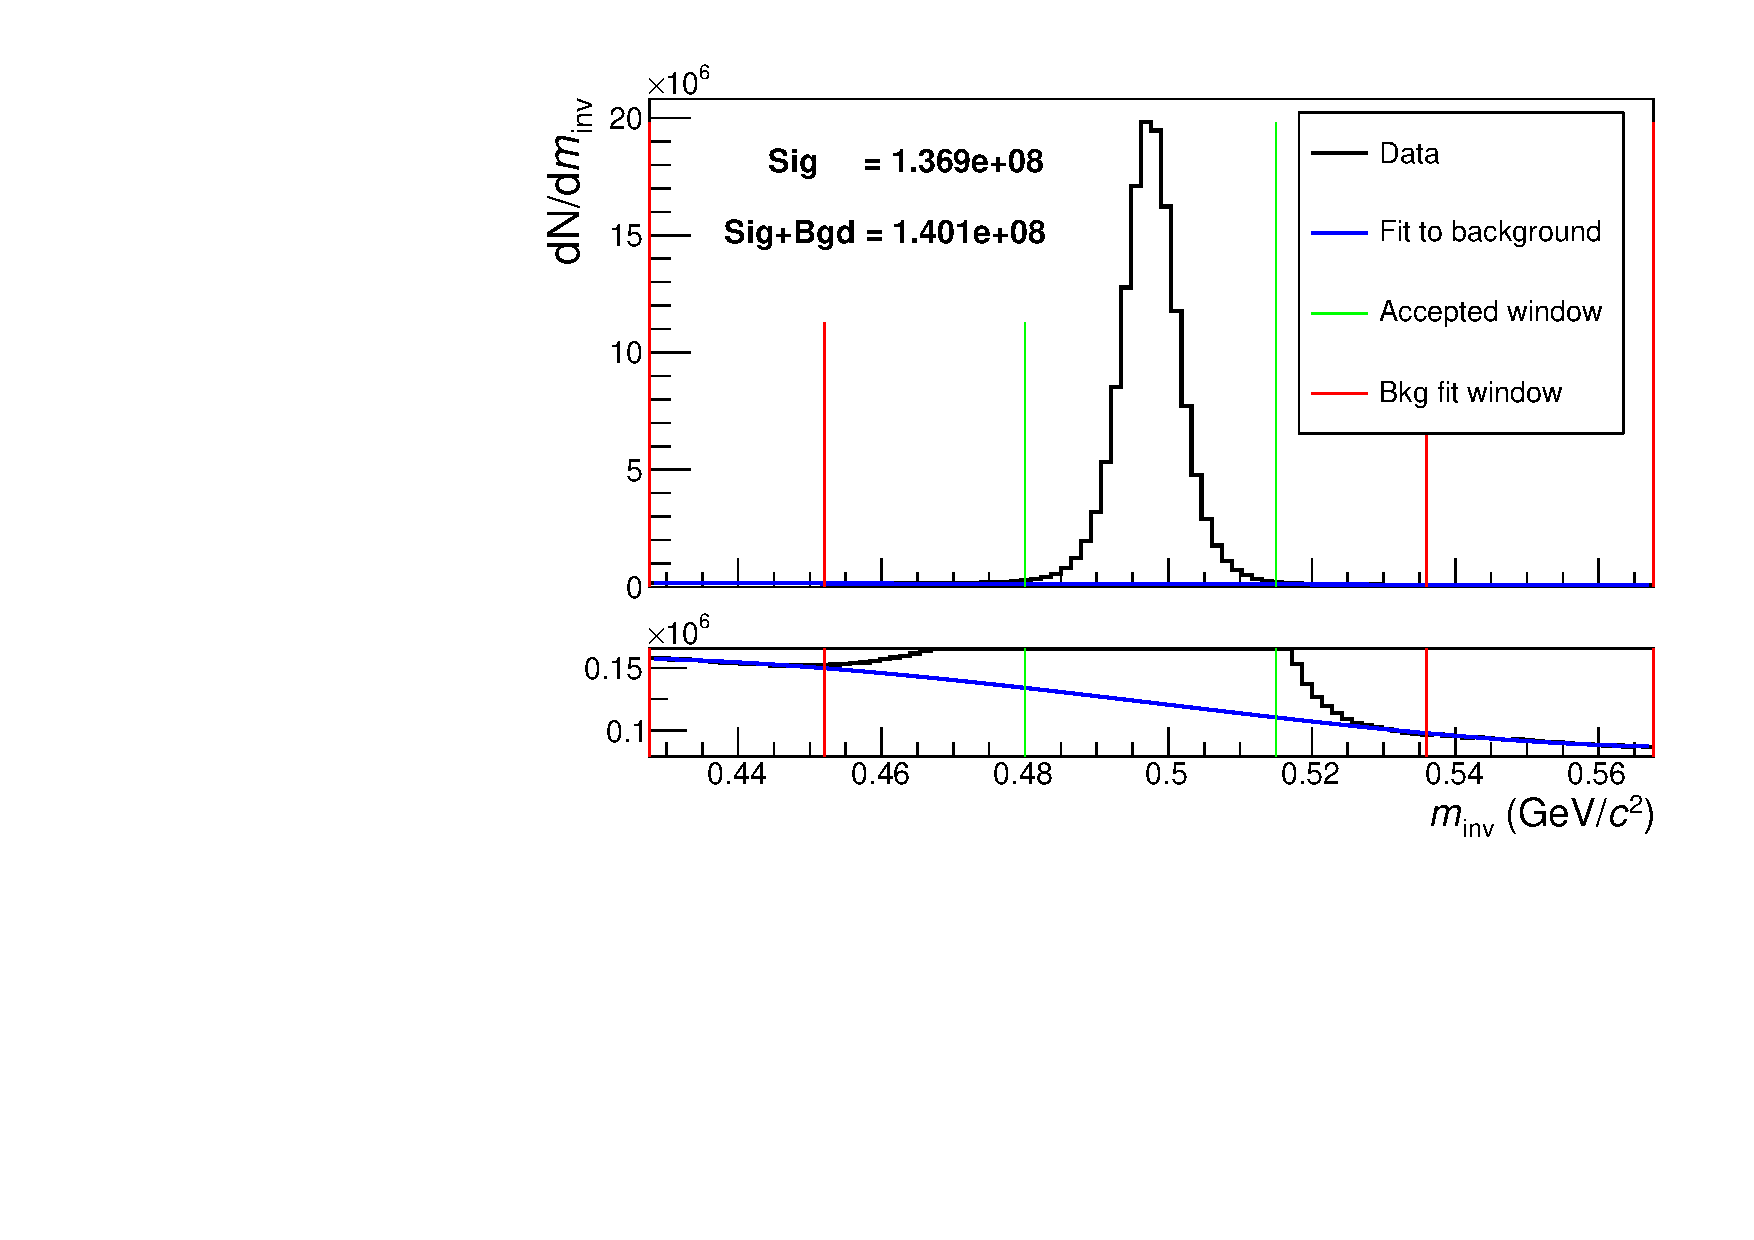
\includegraphics[width=0.49\linewidth]{/home/jesse/Analysis/FemtoAnalysis/LamKPublication/Figures/PDF/K0Purity_LamK0.pdf}}
   %%----overall caption----
   \caption{
-  (Color online) Invariant mass (\minv) distribution of p$\pi^{+}$ pairs showing the \Lam peak \ref{fig:Purity:a}, and of $\pi^{+}\pi^{-}$ pairs showing the \Ks peak \ref{fig:Purity:b}, for \Vz candidates.  
+  (Color online) Invariant mass (\minv) distribution of (a) p$\pi^{+}$ pairs showing the \Lam peak, and of (b) $\pi^{+}\pi^{-}$ pairs showing the \Ks peak, for \Vz candidates.  
   The bottom panels are zoomed to show the background with fit.  
-  The vertical dashed lines represent the \minv cuts used in the analyses, the vertical dotted lines delineate the region over which the background was fit, and the dash-dotted line shows the background fit.
+  The vertical dashed lines represent the \minv restrictions used in the analyses, the vertical dotted lines delineate the region over which the background was fit, and the dash-dotted line shows the background fit.
   }  
   \label{fig:Purity}
 \end{figure}
@@ -477,13 +482,13 @@
 
 
 %************************************************************************************************************************
-\subsection{Pair Construction}
+\subsection{Pair construction}
 \label{PairConstruction}
 
 In order to reduce the contamination to the two-particle correlations due to pairs sharing daughters and to split or merged tracks, two main pair cuts are applied: a shared daughter cut, and an average separation cut.
 The purpose of the shared daughter cut is to ensure the first particle in the pair is unique from the second.  
-For pairs formed of two V$^{0}$s (i.e. \LamKs), this cut is implemented by removing all pairs which share a daughter.  
-For a pair formed of a single \Vz and a charged track (i.e. \LamKpm), the cut removes all pairs in which the charged track is also claimed as a daughter of the \Vz.  
+For pairs formed of two V$^{0}$s (i.e., \LamKs), this cut is implemented by removing all pairs which share a daughter.  
+For a pair formed of a single \Vz and a charged track (i.e., \LamKpm), the cut removes all pairs in which the charged track is also claimed as a daughter of the \Vz.  
 
 
 The purpose of the average separation cut is to remove splitting and merging effects, and it is employed in the following way.  
@@ -495,42 +500,43 @@
 
 %************************************************************************************************************************
 %************************************************************************************************************************
-\section{Analysis Methods}
+\section{Analysis methods}
 \label{sec:AnalysisMethods}
 
 %************************************************************************************************************************
-\subsection{Correlation Function}
+\subsection{Correlation function}
 \label{sec:CorrelationFunction}
-Two-particle correlation functions are built as the ratio of the covariant two-particle and single-particle spectra:
-
-\begin{equation}
-  C^{ab}(\vec{\mathrm{p}_{a}},\vec{\mathrm{p}_{b}}) = \frac{E_{a}E_{b}\frac{dN^{ab}}{d^{3}p_{a}d^{3}p_{b}}}{\big( E_{a}\frac{dN^{a}}{d^{3}p_{a}} \big) \big( E_{b}\frac{dN^{b}}{d^{3}p_{b}} \big)}
+The two-particle correlation function, $C_{ab}(\vec{\mathrm{p}}_{a},\vec{\mathrm{p}}_{b})$, is defined as the ratio of the probability of simultaneously measuring two particles with momenta $p_{a}$ and $p_{b}$, to the product of the single-particle probabilities.
+These probabilities are directly related to the covariant two-particle spectrum, $E_{a}E_{b}\frac{dN_{ab}}{d^{3}p_{a}d^{3}p_{b}}$, and the single-particle spectra, $E_{a(b)}\frac{dN_{a(b)}}{d^{3}p_{a(b)}}$, and the correlation function may be written
+\begin{equation}
+  C_{ab}(\vec{\mathrm{p}}_{a},\vec{\mathrm{p}}_{b}) = \frac{E_{a}E_{b}\frac{dN_{ab}}{d^{3}p_{a}d^{3}p_{b}}}{\big( E_{a}\frac{dN_{a}}{d^{3}p_{a}} \big) \big( E_{b}\frac{dN_{b}}{d^{3}p_{b}} \big)},
 \label{eqn:CfRatioSpectra}
 \end{equation}
-This may be expressed theoretically as in the Koonin-Pratt equation \cite{Koonin:1977fh, Pratt:1990zq}:
-\begin{equation}
- C(\mathbf{k^{*}}) = \int S_{\mathbf{P}}(\mathbf{r^{*}})|\Psi_{\mathbf{k^{*}}}(\mathbf{r^{*}})|^{2}d^{3}\mathbf{r^{*}}
+where $N_{ab}$ is the yield of particle pairs, $E_{a(b)}$ is the energy, $p_{a(b)}$ is the three-momentum, and $N_{a(b)}$ is the yield of particles $a(b)$.
+Theoretically, the correlation function may be expressed as in the Koonin-Pratt equation~\cite{Koonin:1977fh, Pratt:1990zq},
+\begin{equation}
+ C(\mathbf{k^{*}}) = \int S_{\mathbf{P}}(\mathbf{r^{*}})|\Psi_{\mathbf{k^{*}}}(\mathbf{r^{*}})|^{2}d^{3}\mathbf{r^{*}},
 \label{eqn:KooninPrattEqn}
 \end{equation}
 where $\mathbf{k}^{*}$ is the relative momentum of the pair (defined as $\mathbf{k}^{*} = \frac{1}{2}|\mathbf{p}_{1}^{*}-\mathbf{p}_{2}^{*}|$, where $\mathbf{p}_{1}^{*}$ and $\mathbf{p}_{2}^{*}$ are the momenta of the two particles) in the pair rest frame (PRF), $\mathbf{r}^{*}$ is the relative separation in the same frame, $\mathbf{P}$ is the total pair momentum, $S_{\mathbf{P}}(\mathbf{r^{*}})$ is the pair source distribution, and $\Psi_{\mathbf{k^{*}}}(\mathbf{r^{*}})$ is the two-particle wave-function.
-Within the $|\Psi|^{2}$ term is contained the particle interaction information, and therefore the scattering parameters.
-
-In practice, the correlation function is formed experimentally as:
-\begin{equation}
-  C(k^{*}) = \mathcal{N}\frac{A(k^{*})}{B(k^{*})}
+Within the $|\Psi|^{2}$ term the particle interaction information is contained, and therefore the scattering parameters.
+
+In practice, the correlation function is formed experimentally as
+\begin{equation}
+  C(k^{*}) = \mathcal{N}\frac{A(k^{*})}{B(k^{*})},
 \label{eqn:CfExp}
 \end{equation}
 where $A(k^{*})$ is the signal distribution, $B(k^{*})$ is the reference distribution, and $\mathcal{N}$ is a normalization parameter.  
-$B(k^{*})$ is used to divide out the phase-space effects, leaving only the femtoscopic effects in the correlation function. 
+The reference distribution is used to divide out the phase-space effects, leaving only the femtoscopic effects in the correlation function. 
 The normalization parameter is chosen such that the mean value of the correlation function equals unity for \kstar $\in$ [0.32, 0.4] GeV/$c$.
-$A(k^{*})$ is constructed by binning in \kstar pairs from the same event.
-Typically, $B(k^{*})$ is obtained using mixed-event pairs \cite{Kopylov:1974th}, i.e. particles from a given event are paired with those from another event.
-Other techniques exist; most notably, one may use same-event pairs after rotating one particle in the pair by 180$^\circ$ in the transverse plane (see Sec.\ \ref{NonFlatBackground} and App.\ \ref{App:StavMethod} for more details).
+The signal distribution is the same-event distribution of particle pairs.
+Typically, $B(k^{*})$ is obtained using mixed-event pairs~\cite{Kopylov:1974th}, i.e., particles from a given event are paired with those from another event.
+Other techniques exist; most notably, one may use same-event pairs after rotating one particle in the pair by 180$^\circ$ in the transverse plane (see Sec.~\ref{NonFlatBackground} and App.~\ref{App:StavMethod} for more details).
 For this analysis, the typical mixed-event method is utilized, and each event is mixed with five others for the reference distribution construction.
-In order to mix only similar events, events are binned both in primary vertex location (2 cm bin width) and in centrality (5\% bin width), and only events within a given bin are mixed; i.e. only events of like centrality and of like primary vertex location are mixed.
-
-This analysis presents correlation functions for three centrality bins (0--10\%, 10--30\%, and 30--50\%), and is pair transverse momentum ($k_{\mathrm{T}} = \frac{1}{2}|\mathbf{p}_{\mathrm{T,1}}+\mathbf{p}_{\mathrm{T,2}}|$) integrated (i.e. not binned in $k_{\mathrm{T}}$) due to limited statistics.
-The $k_{\mathrm{T}}$-dependences of the three \LamK charge combinations are comparable, so an integrated analysis is acceptable.
+In order to mix similar events, only events of like centrality (within 5\%) and of like primary vertex position (within 2 cm) are mixed.
+
+This analysis presents correlation functions for three centrality percentile ranges (0--10\%, 10--30\%, and 30--50\%), and is pair transverse momentum ($k_{\mathrm{T}} = \frac{1}{2}|\mathbf{p}_{\mathrm{T,1}}+\mathbf{p}_{\mathrm{T,2}}|$) integrated (i.e., no restriction on $k_{\mathrm{T}}$) due to limited data.
+The $k_{\mathrm{T}}$ dependences of the three \LamK charge combinations should be comparable, so an integrated analysis is acceptable.
 The correlation functions were constructed separately for the two different field polarities applied by the ALICE L3 solenoid magnet during the data acquisition.
 These are kept separate during the fitting process, and are combined using a weighted average when plotting, where the weight is the number of numerator pairs in the normalization range.
 
@@ -539,89 +545,97 @@
 \label{sec:ModelingCF}
 
 
-In the absence of the Coulomb interaction, the correlation function can be described analytically with a model derived by Lednick\'y and Lyuboshitz \cite{Lednicky:82}.
-Within the model, the (non-symmetrized) two-particle wave function is expressed as a superposition of a plane wave and diverging spherical wave, and the complex scattering amplitude, $f^{S}(k^{*})$, is evaluated via the effective range approximation
+In the absence of the Coulomb interaction, the correlation function can be described analytically with a model derived by Lednick\'y and Lyuboshitz~\cite{Lednicky:82}.
+Within the model, the (non-symmetrized) two-particle wave function is expressed as a superposition of a plane wave and diverging spherical wave, and the complex scattering amplitude, $f^{S}(k^{*})$, is evaluated via the effective range approximation,
 \begin{equation}
 \begin{aligned}
-f^{S}(k^{*}) = \left( \frac{1}{f^{S}_{0}} + \frac{1}{2}d^{S}_{0}k^{*2} - ik^{*} \right)^{-1}
+f^{S}(k^{*}) = \left( \frac{1}{f^{S}_{0}} + \frac{1}{2}d^{S}_{0}k^{*2} - ik^{*} \right)^{-1},
 \end{aligned}
 \label{eqn:ScatteringParam}
 \end{equation}
 where $f^{S}_{0}$ is the complex s-wave scattering length, $d^{S}_{0}$ is the effective range of the interaction, and $S$ denotes the total spin of the particular pair.
 The sign convention is such that a positive real component of the scattering length, $\Re f_{0}$, represents an attractive interaction, while a negative $\Re f_{0}$ represents a repulsion.
 A spherically symmetric Gaussian distribution with radius $R_{\mathrm{inv}}$  is assumed for the pair emission source in the PRF.
-With these assumptions, utilizing the Koonin-Pratt equation (Eq.\ \ref{eqn:KooninPrattEqn}), the correlation function for non-identical particle pairs with at least one uncharged member is given by \cite{Lednicky:82}
-
+With these assumptions, utilizing the Koonin-Pratt equation (Eq.~\ref{eqn:KooninPrattEqn}), the correlation function for non-identical particle pairs with at least one uncharged member is given by~\cite{Lednicky:82}
 \begin{equation}
 \begin{aligned}
-C(k^{*})_{\mathrm{Lednick\acute{y}}} &= 1 + \sum_{S}\rho_{S}\left[\frac{1}{2}\left|\frac{f^{S}(k^{*})}{R_{\mathrm{inv}}}\right|^2\left(1-\frac{d^{S}_{0}}{2\sqrt{\pi}R_{\mathrm{inv}}}\right)+\frac{2\Re f^{S}(k^{*})}{\sqrt{\pi}R_{\mathrm{inv}}}F_{1}(2k^{*}R_{\mathrm{inv}})-\frac{\Im f^{S}(k^{*})}{R_{\mathrm{inv}}}F_{2}(2k^{*}R_{\mathrm{inv}})\right]
+C(k^{*})_{\mathrm{Lednick\acute{y}}} = &1 + \sum_{S}\rho_{S}\left[\frac{1}{2}\left|\frac{f^{S}(k^{*})}{R_{\mathrm{inv}}}\right|^2\left(1-\frac{d^{S}_{0}}{2\sqrt{\pi}R_{\mathrm{inv}}}\right) \right. \\
+&+ \left. \frac{2\Re f^{S}(k^{*})}{\sqrt{\pi}R_{\mathrm{inv}}}F_{1}(2k^{*}R_{\mathrm{inv}})-\frac{\Im f^{S}(k^{*})}{R_{\mathrm{inv}}}F_{2}(2k^{*}R_{\mathrm{inv}})\right],
 \end{aligned}  
 \label{eqn:LednickyEqn}
 \end{equation}
-
 where $\Re f^{S}(k^{*})$ and $\Im f^{S}(k^{*})$ denote the real and imaginary parts of the complex scattering length, respectively, and $F_{1}$ and $F_{2}$ are the analytic functions.
 The weight factor, $\rho_{S}$ is the normalized emission probability for a state of total spin $S$; in the assumed case of unpolarized emission, $\rho_{S} = (2S+1)/[(2j_{1}+1)(2j_{2}+1)]$, where $j_{1,2}$ are the spins of the particles in the pair.
-The \Lam hyperon is spin-1/2 and K mesons are spin-0, so the \LamK system only has one possible total spin state $S$, and therefore $C(k^{*})$ in Eq.\ \ref{eqn:LednickyEqn} has only a single term.
+The \Lam hyperon is spin-1/2 and K mesons are spin-0, so the \LamK system only has one possible total spin state $S$, and therefore $C(k^{*})$ in Eq.~\ref{eqn:LednickyEqn} has only a single term.
 In the following, the $S$ superscript is dropped from all scattering parameters.
 
 %************************************************************************************************************************
-\subsection{Residual Correlations}
+\subsection{Residual correlations}
 \label{ResidualCorrelations}
 
-The purpose of this analysis is study the interaction and scale of the emitting source of the primary \LamK pairs.
+The purpose of this analysis is to study the interaction and scale of the emitting source of the primary \LamK pairs.
 However, in practice some of the selected particles originate as decay products from other resonances, and some of the final pairs contain a misidentified member.
 In both cases, these contribute to the finally observed correlation function, and obscure its relation to the primary \LamK system.
 The contributions from fake pairs, which contain at least one misidentified member, are assumed to average to unity, in which case they simply attenuate the femtoscopic signal.
-Those pairs whose members originate as daughters from resonances carry information about the parent system.
+Pairs whose members originate as daughters from resonances carry information about the parent system.
 In effect, the correlation between the parents will be visible, although smeared out, in the daughters' signal.
 This is termed a residual correlation resulting from feed-down.  
 As described in the following, the main sources of residual correlations in the \LamK systems result from \Lam hyperons which have decayed from $\Sigma^{0}$, $\Xi^{0}$, and $\Xi^{-}$ parents.
 
-The finally measured correlation function is a combination of the genuine \LamK correlation with contributions from resonances and impurities \cite{Kisiel:2014mma}
+The finally measured correlation function is a combination of the genuine \LamK correlation with contributions from resonances and impurities~\cite{Kisiel:2014mma},
 \begin{equation}
 \begin{aligned}
 \label{eqn:CfwRes} 
- C_{\mathrm{measured}}(k^{*}_{\Lambda\mathrm{K}}) &= 1 + \lambda'_{\Lambda\mathrm{K}}[C_{\Lambda\mathrm{K}}(k^{*}_{\Lambda\mathrm{K}}) - 1] + \sum\limits_{ij}  \lambda'_{ij}[C_{ij}(k^{*}_{\Lambda\mathrm{K}})-1] \\
- \lambda_{ij}' &= \lambda_{\mathrm{Fit}}\lambda_{ij} \\
- \sum\limits_{ij}\lambda_{ij}' &=  \lambda_{\mathrm{Fit}}\sum\limits_{ij}\lambda_{ij} = \lambda_{\mathrm{Fit}}
+ C_{\mathrm{measured}}(k^{*}_{\Lambda\mathrm{K}}) &= 1 + \lambda'_{\Lambda\mathrm{K}}[C_{\Lambda\mathrm{K}}(k^{*}_{\Lambda\mathrm{K}}) - 1] + \sum\limits_{ij}  \lambda'_{ij}[C_{ij}(k^{*}_{\Lambda\mathrm{K}})-1], \\
+\end{aligned} 
+\end{equation}
+with
+\begin{equation}
+\begin{aligned}
+\label{eqn:CfwRes2} 
+ \lambda_{ij}' &= \lambda_{\mathrm{Fit}}\lambda_{ij}, \\
+ \sum\limits_{ij}\lambda_{ij}' &=  \lambda_{\mathrm{Fit}}\sum\limits_{ij}\lambda_{ij} = \lambda_{\mathrm{Fit}},
 \end{aligned} 
 \end{equation}
 where the \LamK term represents the genuine \LamK correlation, and the $ij$ terms denote the contributions from residual feed-down and impurities.
 More specifically, $C_{ij}(k^{*}_{\Lambda\mathrm{K}})$ is the correlation function of the parent system expressed in terms of the relative momentum of the daughter \LamK pair.  
-The $\lambda_{ij}$ parameters serve as weights dictating the relative strength of each component's contribution to the observed signal, and are normalized to unity (i.e. $\sum_{ij} \lambda_{ij} = 1$, where $ij$ includes also the primary \LamK component) \cite{Kisiel:2014mma, Acharya:2018gyz}.
-The individual $\lambda_{ij}$ are fixed (and whose values can be found in Table \ref{tab:LambdaValues_3Res}), but the parameter $\lambda_{\mathrm{Fit}}$ in Eq.\ \ref{eqn:CfwRes} is left free.
-
-
-To obtain the parent correlation function expressed in the relative momentum of the daughter pair, a transform matrix is utilized
-\begin{equation}
-  C_{ij}(k^{*}_{\Lambda\mathrm{K}}) \equiv \frac{\sum\limits_{k^{*}_{ij}} C_{ij}\left(k^{*}_{ij}\right) T\left(k^{*}_{ij},k^{*}_{\Lambda\mathrm{K}}\right)}{\sum\limits_{k^{*}_{ij}} T\left(k^{*}_{ij},k^{*}_{\Lambda\mathrm{K}}\right)}
+The $\lambda_{ij}$ parameters serve as weights dictating the relative strength of each component's contribution to the observed signal, and are normalized to unity (i.e., $\sum_{ij} \lambda_{ij} = 1$, where $ij$ includes also the primary \LamK component)~\cite{Kisiel:2014mma, Acharya:2018gyz}.
+The individual $\lambda_{ij}$ are fixed (and whose values can be found in Table~\ref{tab:LambdaValues_3Res}), but the parameter $\lambda_{\mathrm{Fit}}$ in Eq.~\ref{eqn:CfwRes} is left free.
+
+
+To obtain the parent correlation function expressed in the relative momentum of the daughter pair, a transform matrix is utilized,
+\begin{equation}
+  C_{ij}(k^{*}_{\Lambda\mathrm{K}}) \equiv \frac{\sum\limits_{k^{*}_{ij}} C_{ij}\left(k^{*}_{ij}\right) T\left(k^{*}_{ij},k^{*}_{\Lambda\mathrm{K}}\right)}{\sum\limits_{k^{*}_{ij}} T\left(k^{*}_{ij},k^{*}_{\Lambda\mathrm{K}}\right)},
 \label{eqn:ResidualsTransform}
 \end{equation}
-where $T(k^{*}_{ij},k^{*}_{\Lambda\mathrm{K}})$ is the transform matrix, which is generated with the THERMINATOR 2 \cite{Chojnacki:2011hb} simulation. 
-The transform matrix describes the decay kinematics of the parent system into the daughter, and is essentially an unnormalized probability distribution mapping the \kstar of the parent pair to that of the daughter pair when one or both parents decay (see Ref.\ \cite{Kisiel:2014mma} for more details).
-
-The contribution of a parent system (e.g. $\Sigma^{0}$\KchP) to the daughter correlation function (e.g. \LamKchP) is determined by modeling the parent system's correlation function and running it through the appropriate transform matrix.
+where $T(k^{*}_{ij},k^{*}_{\Lambda\mathrm{K}})$ is the transform matrix, which is generated with the THERMINATOR 2~\cite{Chojnacki:2011hb} simulation. 
+The transform matrix describes the decay kinematics of the parent system into the daughter, and is essentially an unnormalized probability distribution mapping the \kstar of the parent pair to that of the daughter pair when one or both parents decay (see Ref.~\cite{Kisiel:2014mma} for more details).
+
+The contribution of a parent system (e.g., $\Sigma^{0}$\KchP) to the daughter correlation function (e.g., \LamKchP) is determined by modeling the parent system's correlation function and running it through the appropriate transform matrix.
 Since the interactions between these particles are not known, some assumptions must be made.
 When modeling the parent systems, the source radii are assumed to be equal to those of the daughter \LamK systems.
-Furthermore, Coulomb-neutral parent pairs are assumed to share the same scattering parameters as the \LamK daughter pair, and the parent correlation function is modeled using Eq.\ \ref{eqn:LednickyEqn}.
-During the fit process, these source radii and scattering parameters are left free, as described in Sec. \ref{SummarizedFitProcedure}.
-For the \XiKpm parent system, where the constituents interact via both the strong and Coulomb interactions, no analytical expression exists to model the correlation function (see App.\ \ref{App:CoulombFitter}), and the experimental \XiKpm data are used.
+Furthermore, Coulomb-neutral parent pairs are assumed to share the same scattering parameters as the \LamK daughter pair, and the parent correlation function is modeled using Eq.~\ref{eqn:LednickyEqn}.
+During the fit process, these source radii and scattering parameters are left free, as described in Sec.~\ref{SummarizedFitProcedure}.
+For the \XiKpm parent system, where the constituents interact via both the strong and Coulomb interactions, no analytical expression exists to model the correlation function (see App.~\ref{App:CoulombFitter}), and the experimental \XiKpm data are used.
 The \XiKpm correlation function is dominated by the contribution from the Coulomb interaction, and consistent final fit results are obtained when modeling \XiKpm the system with a Coulomb-only scenario, in which the strong interaction is assumed to be negligible, instead of using the experimental data.
 
 
 
 The $\lambda_{ij}$ parameters dictate the relative strength of each contribution to the correlation function, and can be estimated using the THERMINATOR 2 and HIJING simulations.
-More specifically, a $\lambda_{ij}$ parameter is estimated as the total number of \LamK pairs in the experimental sample originating from $ij$ ($N_{ij}$) divided by the total number of \LamK pairs.
-The number of detected \LamK pairs involves both the raw yields and the reconstruction efficiencies.
-The reconstruction efficiencies ($RE_{ij}$) are estimated with MC HIJING data, which have been run through GEANT to simulate the detector response.
+More specifically, a $\lambda_{ij}$ parameter is estimated as the total number of \LamK pairs in the sample originating from source $ij$ ($N_{ij}$) divided by the total number of \LamK pairs.
+For a given \LamK source, the number of detected pairs depends on both the raw yield and the reconstruction efficiency.
+The reconstruction efficiencies ($RE_{ij}$) are estimated with HIJING simulations using GEANT3 to model particle transport through the detector.
 HIJING events are generated from a superposition of PYTHIA p-p collisions, and lack the strangeness saturation of a fully thermalized medium.
 As a result, HIJING is unreliable in providing the yields needed for this analysis, and, instead, the yields are estimated with the THERMINATOR 2 simulation ($N_{ij}^{\scaleto{THERM}{3pt}}$).
-The number of \LamK pairs is then estimated as the product of the yield with the reconstruction efficiency, $N_{ij} = N_{ij}^{\scaleto{THERM}{3pt}}RE_{ij}^{\scaleto{HIJING}{3pt}}$.
-
+The number of \LamK pairs from source $ij$ is then estimated as the product of the yield with the associated reconstruction efficiency, $N_{ij} = N_{ij}^{\scaleto{THERM}{3pt}}RE_{ij}^{\scaleto{HIJING}{3pt}}$.
+Finally, the $\lambda_{ij}$ are estimated as
+\begin{equation}
+\lambda_{ij} = \frac{N_{ij}}{N_{Total}} = \frac{N_{ij}^{\scaleto{THERM}{3pt}}RE_{ij}^{\scaleto{HIJING}{3pt}}}{\sum\limits_{\alpha\beta} N_{\alpha\beta}^{\scaleto{THERM}{3pt}}RE_{\alpha\beta}^{\scaleto{HIJING}{3pt}}}.
+\end{equation}
 
 
 Femtoscopic analyses are sensitive to the pair emission structure at kinetic freeze-out.
-Therefore, in the eyes of femtoscopy, any particle born from a resonance decay before last rescattering is seen as primary.
+Therefore, within femtoscopy, any particle which originates from a resonance decay before last rescattering is considered primary.
 The THERMINATOR 2 simulation shows that, aside from primaries, the \Lam hyperons and K mesons decay from a large number of resonances ($\sim$50 \Lam parent species, and $\sim$70 K parent species), and the most significant contributing pair systems are $\Sigma^{0}$K, $\Xi^{-}$K, $\Xi^{0}$K, $\Sigma^{*+}$K, $\Sigma^{*-}$K, $\Sigma^{*0}$K, $\Lambda\mathrm{K}^{*}$, $\Sigma^{0}\mathrm{K}^{*}$, $\Xi^{-}\mathrm{K}^{*}$, and $\Xi^{0}\mathrm{K}^{*}$.
 However, the simulation does not include a hadronic rescattering phase, and not all of the aforementioned pair systems will survive until kinetic freeze-out.
 The systems resulting from electromagnetic or weak decays ($\Sigma^{0}$, $\Xi^{-}$, and $\Xi^{0}$) will survive long after kinetic freeze-out, and will contribute residual signals to the \LamK correlation functions.
@@ -631,11 +645,11 @@
 Changing $c\tau$ only moderately affects the $\lambda_{ij}$ parameters, and the effect is included in the estimation of the systematic uncertainties.
 In order for a pair to be considered primary, both particles in the pair must be considered primary. 
 If either parent has $\tau > \tau_{\mathrm{max}}$, the daughter pair contributes to the ``Other" category when calculating $\lambda$ parameters.
-For this hodgepodge of pair systems, all with different two-particle interactions and single-particle source distributions, we assume the net correlation effect averages to unity.
+For this mixture of pair systems, all with different two-particle interactions and single-particle source distributions, the net correlation effect is assumed to average to unity.
 
 
 Residual contributions from $\Sigma^{0}$, $\Xi^{0}$, $\Xi^{-}$ are accounted for in the fit.
-The $\lambda_{ij}$ values used can be found in Table \ref{tab:LambdaValues_3Res}, which also included values for ``Other'' and ``Fakes''.  
+The $\lambda_{ij}$ values used can be found in Table~\ref{tab:LambdaValues_3Res}, which also included values for ``Other'' and ``Fakes''.  
 The ``Other'' category contains pairs which are not considered primary, and which do not originate from the residual contributors accounted for in the fit.  
 The ``Fakes'' category represents pairs that are mistakenly identified as \LamK.  
 To estimate the $\lambda_{\mathrm{Fakes}}$ value, the number of fake pairs is assumed to be equal to the total number of simulated pairs multiplied by $(1-PP_{\Lambda\mathrm{K}})/PP_{\Lambda\mathrm{K}}$, where $PP_{\Lambda\mathrm{K}}$ is the \LamK pair purity, estimated as the product of the two single-particle purities ($PP_{\Lambda\mathrm{K}} = P_{\Lambda}P_{\mathrm{K}}$).
@@ -645,6 +659,7 @@
 
 \begin{table}[htbp]
  \centering
+ \caption{Weight parameters ($\lambda_{ij}$) for the individual components of the \LamK correlation functions.}
  \renewcommand{\arraystretch}{1.2}
 
  \begin{tabular}{|c|cV{4.0}c|cV{4.0}c|cV{4.0}c|c|}
@@ -674,55 +689,52 @@
   \multicolumn{2}{c|}{} & Fakes & 0.048 & Fakes & \multicolumn{1}{c|}{0.048} & \multicolumn{2}{c}{} \\
   \clineB{3-6}{3.0} 
  \end{tabular}
- \caption{$\lambda$ values for the individual components of the \LamK correlation functions.}
+ %\caption{$\lambda$ values for the individual components of the \LamK correlation functions.}
  \label{tab:LambdaValues_3Res}
 \end{table}
 
 %************************************************************************************************************************
-\subsection{Momentum Resolution Corrections}
+\subsection{Momentum resolution corrections}
 \label{MomentumResolutionCorrections}
 
 Finite track momentum resolution causes the reconstructed momentum of a particle to smear around the true value.
 This, of course, also holds true for \Vz particles.
 The effect is propagated up to the pairs of interest, which causes the reconstructed relative momentum (\krec) to differ from the true momentum (\ktrue).
-The effects of finite momentum resolution are accounted for through the use of a response matrix generated with MC HIJING data.
+The effects of finite momentum resolution are accounted for through the use of a response matrix generated with HIJING simulations.
 With this approach, the resolution correction is applied on-the-fly during the fitting process by propagating the theoretical (fit) correlation function through the response matrix, according to
 \begin{equation}
-  C_{\mathrm{fit}}(k^{*}_{\mathrm{Rec}}) = \dfrac{\sum\limits_{k^{*}_{\mathrm{True}}}M_{k^{*}_{\mathrm{Rec}},k^{*}_{\mathrm{True}}}C_{\mathrm{fit}}(k^{*}_{\mathrm{True}})}{\sum\limits_{k^{*}_{\mathrm{True}}}M_{k^{*}_{\mathrm{Rec}},k^{*}_{\mathrm{True}}}}
+  C_{\mathrm{fit}}(k^{*}_{\mathrm{Rec}}) = \dfrac{\sum\limits_{k^{*}_{\mathrm{True}}}M_{k^{*}_{\mathrm{Rec}},k^{*}_{\mathrm{True}}}C_{\mathrm{fit}}(k^{*}_{\mathrm{True}})}{\sum\limits_{k^{*}_{\mathrm{True}}}M_{k^{*}_{\mathrm{Rec}},k^{*}_{\mathrm{True}}}},
 \label{eqn:MomResCorrection}
 \end{equation}
-where $M_{k^{*}_{\mathrm{Rec}},k^{*}_{\mathrm{True}}}$ is the response matrix, $C_{\mathrm{fit}}(k^{*}_{\mathrm{True}})$ is the fit binned in \ktrue, and the denominator normalizes the result.
-Equation \ref{eqn:MomResCorrection} describes that, for a given \krec bin, the observed value of $C(k^{*}_{\mathrm{Rec}})$ is a weighted average of all $C(k^{*}_{\mathrm{True}})$ values, where the weights are the normalized number of counts in the \mbox{$[k^{*}_{\mathrm{Rec}}, k^{*}_{\mathrm{True}}]$} bin.
-
-
-%************************************************************************************************************************
-\subsection{Non-Femtoscopic Background}
+where $M_{k^{*}_{\mathrm{Rec}},k^{*}_{\mathrm{True}}}$ is the response matrix, $C_{\mathrm{fit}}(k^{*}_{\mathrm{True}})$ is the fit as a function of \ktrue, and the denominator normalizes the result.
+Equation~\ref{eqn:MomResCorrection} describes that, for a given \krec, the observed value of $C(k^{*}_{\mathrm{Rec}})$ is a weighted average of all $C(k^{*}_{\mathrm{True}})$ values, where the weights are the normalized number of counts in the \mbox{$[k^{*}_{\mathrm{Rec}}, k^{*}_{\mathrm{True}}]$} bin.
+
+
+%************************************************************************************************************************
+\subsection{Non-femtoscopic background}
 \label{NonFlatBackground}
 
-A significant non-femtoscopic background is observed in all of the studied \LamK correlations which increases with decreasing centrality, is the same amongst all \LamKpm pairs, and is more pronounced in the \LamKs system (the difference in \LamKpm and \LamKs backgrounds is due mainly to a difference in kinematic cuts).  
-The background is due primarily to particle collimation associated with elliptic flow, and results from mixing events with unlike event-plane angles\footnote[1]
-{
-An attempt was made to decrease the background by binning events in $\Psi_{\mathrm{EP}}$, but only a small reduction in the signal was achieved due to the limited event-plane resolution.
-}\cite{Kisiel:2017}.
-The effect produces the observed suppression at intermediate-\kstar, and should also lead to an enhancement at low-\kstar.
-The behavior of the non-femtoscopic background is needed in the low-\kstar signal region, but a clean view of it is only possible outside of such a region.
-
-The THERMINATOR 2 simulation has been shown to reproduce the background features in a $\pi$K analysis \cite{Kisiel:2017}. 
+A significant non-femtoscopic background is observed in all of the studied \LamK correlations, which increases with decreasing centrality, is the same amongst all \LamKpm pairs, and is more pronounced in the \LamKs system (the difference in \LamKpm and \LamKs backgrounds is due mainly to a difference in kinematic selection criteria).  
+The background is primarily due to particle collimation associated with elliptic flow, and results from mixing events with unlike event planes~\cite{Kisiel:2017}.
+The effect produces the observed suppression at intermediate \kstar, and should also lead to an enhancement at low \kstar.
+The behavior of the non-femtoscopic background is needed in the low \kstar femtoscopic signal region, but an isolated view of it is only possible outside of such a region.
+
+The THERMINATOR 2 simulation has been shown to reproduce the background features in a $\pi$K analysis~\cite{Kisiel:2017}. 
 The simulation does not include any final-state effects, but they can be introduced by weighting the numerator pairs with the modulus squared of the appropriate two-particle wave-function when building the signal distributions. 
 For the present purpose, only the behavior of the non-femtoscopic background is desired, and unit weights are used.
-Figure \ref{fig:BgdswTHERM} shows the THERMINATOR 2 simulation (open triangles) together with experimental data (closed circles).  
-The figure also shows a 6$^{\mathrm{th}}$-order polynomial fit to the simulation (dashed curves), as well as the fit polynomial scaled to match the data (solid curves).
+Figure~\ref{fig:BgdswTHERM} shows the THERMINATOR 2 simulation together with experimental data.  
+The figure also shows a 6$^{\mathrm{th}}$-order polynomial fit to the simulation, as well as the fit polynomial scaled to match the data.
 
 The THERMINATOR 2 simulation offers a good description of the non-femtoscopic backgrounds in the \LamK systems, and can be used in a quantitative fashion to help fit the data.
-More specifically, the non-femtoscopic backgrounds are modeled by 6$^{\mathrm{th}}$-order polynomial fits to THERMINATOR 2 simulation
-\begin{equation}
-F_{\scaleto{THERM.\; Bgd}{6pt}}(k^{*}) = a{k^{*}}^{6}+ b{k^{*}}^{5} + c{k^{*}}^{4} + d{k^{*}}^{3} + e{k^{*}}^{2} + fk^{*} + g
+More specifically, the non-femtoscopic backgrounds are modeled by 6$^{\mathrm{th}}$-order polynomial fits to THERMINATOR 2 simulation,
+\begin{equation}
+F_{\scaleto{THERM.\; Bgd}{6pt}}(k^{*}) = a{k^{*}}^{6}+ b{k^{*}}^{5} + c{k^{*}}^{4} + d{k^{*}}^{3} + e{k^{*}}^{2} + fk^{*} + g,
 \end{equation}
 where the linear term coefficient is fixed to zero ($f=0$), and one polynomial is fit for each centrality class and \LamK charge combination.
-The coefficients of each polynomial are set before use with the experimental data by fitting to the THERMINATOR 2 simulation, shown in Fig.\ \ref{fig:BgdswTHERM}.
+The coefficients of each polynomial are set before application with the experimental data by fitting to the THERMINATOR 2 simulation, shown in Fig.~\ref{fig:BgdswTHERM}.
 The extracted polynomial is adjusted to best describe the experimental data by introducing a scale factor and a vertical shift,
 \begin{equation}
-F_{\scaleto{Bgd}{6pt}}(k^{*}) = \alpha\cdot F_{\scaleto{THERM.\; Bgd}{6pt}}(k^{*}) + \beta
+F_{\scaleto{Bgd}{6pt}}(k^{*}) = \alpha\cdot F_{\scaleto{THERM.\; Bgd}{6pt}}(k^{*}) + \beta,
 \end{equation}
 where $\alpha$ and $\beta$ are determined by fitting to the data in the region $0.32 < k^{*} < 0.80$ GeV/$c$; during the fit of the low-\kstar signal region, the background is fixed.
 In all cases, the non-femtoscopic background correction was applied as a scale factor.
@@ -747,55 +759,59 @@
 The background may be effectively reduced by forming the reference distribution ($B(k^{*})$) with the ``Stavinskiy method".
 With the Stavinskiy method, mixed-event pairs are not used for the reference distribution; instead, same-event pseudo-pairs, formed by rotating one particle in a real pair by 180$^\circ$ in the transverse plane, are used.  
 This rotation rids the pairs of any femtoscopic correlation, while maintaining correlations due to elliptic flow (and other suitably symmetric contributors).
-The flattening effect of the method on the \LamKchP correlation functions can be seen in the appendix, in Fig.\ \ref{fig:StavCfs_Correct_LamKchP}.
+The flattening effect of the method on the \LamKchP correlation functions can be seen in the appendix, in Fig.~\ref{fig:StavCfs_Correct_LamKchP}.
 
 %************************************************************************************************************************
 \subsection{Summarized correlation function construction}
 \label{SummarizedFitProcedure}
 
 The parameters included in the generation of a correlation function are: $\lambda_{\mathrm{Fit}}$, $R$, $f_{0}$ ($\Re f_{0}$ and $\Im f_{0}$ separately), $d_{0}$, and normalization $\mathcal{N}$.
-For the fit, a given pair and its conjugate (e.g. \LamKchP and \ALamKchM) share scattering parameters ($\Re f_{0}$, $\Im f_{0}$, $d_{0}$), and the three distinct analyses (\LamKchP, \LamKchM, and \LamKs) are assumed to have scattering parameters unique from each other.
-The pair emission source for a given centrality class is assumed similar between all analyses; therefore, for each centrality, all \LamK analyses share a common radius parameter.
-For each centrality class, a single $\lambda_{\mathrm{Fit}}$ parameter (see Eq.\ \ref{eqn:CfwRes}) is shared amongst all.
-Finally, each correlation function has a unique normalization parameter.
-
-All correlation functions are normalized in the range 0.32 $< k^{*} <$ 0.40 GeV/$c$, and fit in the range 0.0 $< k^{*} <$ 0.30 GeV/$c$.
+For the fit, a given pair and its conjugate (e.g., \LamKchP and \ALamKchM) share scattering parameters ($\Re f_{0}$, $\Im f_{0}$, $d_{0}$), and the three distinct analyses (\LamKchP, \LamKchM, and \LamKs) are assumed to have scattering parameters unique from each other.
+The pair emission source for a given centrality class is assumed similar among all analyses; therefore, for each centrality, all \LamK analyses share a common radius parameter.
+For each centrality class, a single $\lambda_{\mathrm{Fit}}$ parameter (see Eq.~\ref{eqn:CfwRes}) is shared amongst all.
+Finally, each correlation function has a unique normalization parameter, $\mathcal{N}$.
+
+All experimental correlation functions are normalized in the range 0.32 $< k^{*} <$ 0.40 GeV/$c$, and fit in the range 0.0 $< k^{*} <$ 0.30 GeV/$c$.
 For the \LamKchM analysis, the region 0.19 $< k^{*} <$ 0.23 GeV/$c$ was excluded from the fit to exclude the bump caused by the $\Omega^{-}$ resonance.
-For each pair system, contributions from three residual contributors are accounted for, as discussed in Sec.\ \ref{ResidualCorrelations}, and whose individual $\lambda$ values are listed in Table \ref{tab:LambdaValues_3Res}.
-Effects of finite track momentum resolution are also accounted for, as outlined in Sec.\ \ref{MomentumResolutionCorrections}.
-The non-femtoscopic backgrounds are modeled using the THERMINATOR 2 simulation, as described in Sec.\ \ref{NonFlatBackground}.
-A log-likelihood fit function is used as the statistic quantifying the quality of the fit \cite{Lisa:2005dd}.
+For each pair system, contributions from three residual contributors are accounted for, as discussed in Sec.~\ref{ResidualCorrelations}, and whose individual $\lambda$ values are listed in Table~\ref{tab:LambdaValues_3Res}.
+Effects of finite track momentum resolution are also accounted for, as outlined in Sec.~\ref{MomentumResolutionCorrections}.
+The non-femtoscopic backgrounds are modeled using the THERMINATOR 2 simulation, as described in Sec.~\ref{NonFlatBackground}.
+A log-likelihood fit function is used as the statistic quantifying the quality of the fit~\cite{Lisa:2005dd}.
 
 To summarize, the complete fit function is constructed as follows.
-The uncorrected, primary, correlation function, $C_{\Lambda\mathrm{K}}(k^{*}_{\mathrm{\Lambda K,\,True}})$, is constructed using Eq.\ \ref{eqn:LednickyEqn}.
-The correlation functions describing the parent systems which contribute residually, $C_{ij}(k^{*}_{ij,\,\mathrm{True}})$, are obtained using Eq.\ \ref{eqn:LednickyEqn} for Coulomb-neutral pairs or experimental data for \XiKpm contributions.
-The residual contributions are then found by running each parent correlation function through the appropriate transform matrix, via Eq.\ \ref{eqn:ResidualsTransform}.
-The primary and residual correlations are combined, via Eq.\ \ref{eqn:CfwRes} with Tab.\ \ref{tab:LambdaValues_3Res}, to form $C'_{Fit}$(\ktrue).
-Corrections are applied to account for momentum resolution effects using Eq.\ \ref{eqn:MomResCorrection}, to obtain $C'_{\mathrm{Fit}}(k^{*}_{\mathrm{Rec}})$.
-Finally, the non-femtoscopic background correction, $F_{\mathrm{Bgd}}(k^{*}_{\mathrm{Rec}})$ is applied and the final fit function is obtained 
-\begin{equation}
-C_{\mathrm{Fit}}(k^{*}_{\mathrm{Rec}}) = \mathcal{N}\cdot F_{\mathrm{Bgd}}(k^{*}_{\mathrm{Rec}})\cdot C'_{\mathrm{Fit}}(k^{*}_{\mathrm{Rec}})
+The uncorrected, primary, correlation function, $C_{\Lambda\mathrm{K}}(k^{*}_{\mathrm{\Lambda K,\,True}})$, is constructed using Eq.~\ref{eqn:LednickyEqn}.
+The correlation functions describing the parent systems which contribute residually, $C_{ij}(k^{*}_{ij,\,\mathrm{True}})$, are obtained using Eq.~\ref{eqn:LednickyEqn} for Coulomb-neutral pairs or experimental data for \XiKpm contributions.
+The residual contributions are then found by running each parent correlation function through the appropriate transform matrix, via Eq.~\ref{eqn:ResidualsTransform}.
+The primary and residual correlations are combined, via Eq.~\ref{eqn:CfwRes} with Tab.~\ref{tab:LambdaValues_3Res}, to form $C'_{Fit}$(\ktrue).
+Corrections are applied to account for momentum resolution effects using Eq.~\ref{eqn:MomResCorrection}, to obtain $C'_{\mathrm{Fit}}(k^{*}_{\mathrm{Rec}})$.
+Finally, the non-femtoscopic background correction, $F_{\mathrm{Bgd}}(k^{*}_{\mathrm{Rec}})$, is applied and the final fit function is obtained,
+\begin{equation}
+C_{\mathrm{Fit}}(k^{*}_{\mathrm{Rec}}) = \mathcal{N}\cdot F_{\mathrm{Bgd}}(k^{*}_{\mathrm{Rec}})\cdot C'_{\mathrm{Fit}}(k^{*}_{\mathrm{Rec}}),
 \end{equation}
 where $\mathcal{N}$ is a normalization parameter.
-$C'_{\mathrm{Fit}}(k^{*}_{\mathrm{Rec}})$ includes all components of the correlation function weighted by the appropriate $\lambda_{ij}$ (see Sec.\ \ref{ResidualCorrelations}) parameters and has been corrected for momentum resolution effects (see Sec.\ \ref{MomentumResolutionCorrections}).
+$C'_{\mathrm{Fit}}(k^{*}_{\mathrm{Rec}})$ includes all components of the correlation function weighted by the appropriate $\lambda_{ij}$ (see Sec.~\ref{ResidualCorrelations}) parameters and has been corrected for momentum resolution effects (see Sec.~\ref{MomentumResolutionCorrections}).
 
 %************************************************************************************************************************
 \subsection{Systematic uncertainties}
 \label{SysErrs}
 
-To quantify the systematic errors on the data, all correlation functions built using all varied cut values were bin-by-bin averaged, and the resulting variance of each bin was taken as the systematic error.  
-The cuts included in the systematic study, as well as the values used in the variations, are shown in Tab.\ \ref{tab:LamKSystematics}.  
-Note, the central value corresponds to that used in the analysis.
-Similarly, the fit parameters extracted from all of these correlation functions were averaged, and the resulting variances were taken as the systematic errors for the fit parameters.
-Additionally, for the extracted fit parameters, a systematic analysis was done on the fit method through varying the \kstar fit range, varying the modeling of the non-femtoscopic background, as well as varying $\tau_{\mathrm{max}}$ defining the primary category in the treatment of residual correlations.
-The choice of \kstar fit range was varied by $\pm$ 25\%. 
-As previously stated, the non-femtoscopic backgrounds are modeled with a polynomial fit to the THERMINATOR 2 simulation, scaled to match the data.
-To study the contribution of this choice to the systematic errors, the backgrounds of all of the systems were modeled by fitting to the data with a linear, quadratic, and Gaussian form.
+To estimate the systematic uncertainties in the analysis, the selection criteria were varied, and correlation functions and fit results were obtained for each variation.
+The selection criteria included in the systematic study, as well as the values used in the variations, are shown in Tab.~\ref{tab:LamKSystematics}.  
+Note, in each case, the central value corresponds to that used in the analysis.
+To quantify the systematic uncertainties on the data, the correlation functions from each variation of the selection criteria were averaged, and the standard deviations were calculated for each data point.
+The systematic uncertainties of the correlation functions were set to these calculated standard deviations.
+
+A similar process was followed for estimating the systematic uncertainties of the extracted fit parameters.
+Namely, the extracted fit parameters from each variation were averaged, and the resulting standard deviations taken as the systematic uncertainties.
+Additionally, a systematic analysis was done on the fit method through varying the \kstar fit range, varying the modeling of the non-femtoscopic background, as well as varying $\tau_{\mathrm{max}}$ in the treatment of residual correlations.
+The choice of \kstar fit range was varied by $\pm$ 25\%.
+In addition to modeling with a polynomial fit to the THERMINATOR 2 simulation, the backgrounds of all of the systems were modeled by fitting to the data with a linear, quadratic, and Gaussian form.
 Finally, $\tau_{\mathrm{max}}$ was varied from the default value of $\tau_{\mathrm{max}} = 10$ fm/$c$ down to $\tau_{\mathrm{max}} = 6$ fm/$c$ and up to $\tau_{\mathrm{max}} = 15$ fm/$c$.
-The resulting uncertainties in the extracted parameter sets were combined with the uncertainties arising from the particle and pair cuts.
+The resulting uncertainties in the extracted parameter sets were combined with the uncertainties arising from the variations of the selection criteria.
 
 \begin{table}[htbp]
  \centering 
+ \caption[\LamK systematics]{Selection parameter variation for the study of systematic uncertainties in the analysis. In the table, the shorthand used is as follows: $PA$ = pointing angle; PV = primary vertex; DCA = distance of closest approach; $\overline{\Delta\mathbf{r}}$ = average separation}
   \renewcommand{\arraystretch}{1.2}
   \begin{tabular}{l|r}
    \hlineB{3.0} 
@@ -845,7 +861,7 @@
    
   \end{tabular}
 % \end{minipage}
- \caption[\LamK systematics]{\LamK systematics. In the table, the shorthand used is as follows: $PA$ = pointing angle; PV = primary vertex; DCA = distance of closest approach; $\overline{\Delta\mathbf{r}}$ = average separation}
+ %\caption[\LamK systematics]{\LamK systematics. In the table, the shorthand used is as follows: $PA$ = pointing angle; PV = primary vertex; DCA = distance of closest approach; $\overline{\Delta\mathbf{r}}$ = average separation}
  \label{tab:LamKSystematics} 
 \end{table}
 
@@ -858,15 +874,14 @@
 \section{Results}
 \label{sec:Results}
 
-Figure \ref{fig:LamKFits_3Res} shows the \LamK data with fits for all studied centrality bins (0--10\%, 10--30\%, and 30--50\%). 
-All six \LamK systems (\LamKchP, \ALamKchM, \LamKchM, \ALamKchP, \LamKs, \ALamKs) are fit simultaneously across all centralities, with a single radius and normalization $\lambda_{\mathrm{Fit}}$ parameter for each centrality bin.
-Scattering parameters ($\Re f_{0}$, $\Im f_{0}$, $d_{0}$) are shared between pair-conjugate systems, but assumed unique between the different \LamK charge combinations (i.e. a parameter set describing the \LamKchP \& \ALamKchM system, a second set describing the \LamKchM \& \ALamKchP system, and a third for the \LamKs \& \ALamKs system).
+Figure~\ref{fig:LamKFits_3Res} shows the \LamK data with fits for all studied centrality percentile intervals (0--10\%, 10--30\%, and 30--50\%). 
+All six \LamK systems (\LamKchP, \ALamKchM, \LamKchM, \ALamKchP, \LamKs, \ALamKs) are fit simultaneously across all centralities, with a single radius and normalization $\lambda_{\mathrm{Fit}}$ parameter for each centrality interval.
+Scattering parameters ($\Re f_{0}$, $\Im f_{0}$, $d_{0}$) are shared between pair-conjugate systems, but assumed unique among the different \LamK charge combinations (i.e., a parameter set describing the \LamKchP \& \ALamKchM system, a second set describing the \LamKchM \& \ALamKchP system, and a third for the \LamKs \& \ALamKs system).
 Each correlation function receives a unique normalization parameter.
-The fits are corrected for finite momentum resolution effects, non-femtoscopic backgrounds, and residual correlations resulting from the feed-down from resonances.
-In Fig.\ \ref{fig:LamKFits_3Res}, lines represent statistical errors, while boxes represent systematic errors.  
-The dotted curve shows the primary (\LamK) contribution to the fit (i.e. $1 + \lambda'_{\Lambda\mathrm{K}}C_{\Lambda\mathrm{K}}(k^{*}_{\Lambda\mathrm{K}})$ in Eq.\ \ref{eqn:CfwRes}), the dashed curve shows the fit to the non-femtoscopic background, and the solid curve shows the final fit, with all residual contributions included and after all corrections have been applied.
+The fits are corrected for finite momentum resolution effects, non-femtoscopic backgrounds, and residual correlations resulting from the feed-down from resonances.  
+The figure shows the primary (\LamK) contribution to the fit (i.e., $1 + \lambda'_{\Lambda\mathrm{K}}C_{\Lambda\mathrm{K}}(k^{*}_{\Lambda\mathrm{K}})$ in Eq.~\ref{eqn:CfwRes}), the fit to the non-femtoscopic background, and the final fit, with all residual contributions included and after all corrections have been applied.
 The extraction of the primary \LamK component is the purpose of this study.
-The figure demonstrates that the final fit function is similar to the primary \LamK component, with the largest differences between the two observed in the 30-50\% centrality bin due mainly to the large contribution of the non-femtoscopic background.
+The figure demonstrates that the final fit function is similar to the primary \LamK component, with the largest differences between the two observed in the 30--50\% centrality interval due mainly to the large contribution of the non-femtoscopic background.
 
 \begin{figure}[h!]
   \centering
@@ -876,8 +891,9 @@
   {
   (Color online) Fit results for the \LamK data, with pair and conjugate combined.
   The \LamKchP$\oplus$\ALamKchM data are shown in the left column, the \LamKchM$\oplus$\ALamKchP in the middle, and the \LamKs$\oplus$\ALamKs in the right. 
-  Rows differentiate the different centrality bins (0--10\% in the top, 10--30\% in the middle, and 30--50\% in the bottom).
-  See text for further details.
+  Rows differentiate the different centrality intervals (0--10\% in the top, 10--30\% in the middle, and 30--50\% in the bottom).
+  Lines represent statistical uncertainties, while boxes represent systematic uncertainties.
+  The dotted curve shows the primary (\LamK) contribution to the fit, the dashed curve shows the fit to the non-femtoscopic background, and the solid curve shows the final fit.
  }
   \label{fig:LamKFits_3Res}
 \end{figure}
@@ -888,90 +904,89 @@
   \caption[Extracted Scattering Parameters]
   {
   (Color online) Extracted fit parameters for all of the \LamK systems.  
-  [Left]: $\Im f_{0}$ vs. $\Re f_{0}$, together with $d_{0}$ to the right for the \LamKchP (circles), \LamKchM (squares) and \LamKs (triangles) systems.  
-  [Right]: $\lambda$ vs. Radius for the 0--10\% (circles), 10--30\% (squares), and 30--50\% (triangles) centrality bins.  
+  [Left]: $\Im f_{0}$ and $\Re f_{0}$, together with $d_{0}$ to the right for the \LamKchP (circles), \LamKchM (squares) and \LamKs (triangles) systems.  
+  [Right]: $\lambda$ and radius parameters for the 0--10\% (circles), 10--30\% (squares), and 30--50\% (triangles) centrality intervals.  
   In the fit, all \LamK systems share common radii.
-  The cross ([A] = Ref.\ \cite{Liu:2006xja}) and X symbols ([B] = Ref.\ \cite{Mai:2009ce}) points show theoretical predictions made using chiral perturbation theory.
+  The cross~\cite{Liu:2006xja} and X~\cite{Mai:2009ce} points show theoretical predictions made using chiral perturbation theory.
   }
   \label{fig:ScattParams_3Res}
 \end{figure}
 
-Figure \ref{fig:ScattParams_3Res} (left) summarizes the extracted \LamK scattering parameters, and includes theoretical predictions made using chiral perturbation theory \cite{Liu:2006xja,Mai:2009ce}.
-The predictions of Ref.\ \cite{Liu:2006xja} do not distinguish the K\Lam and K\ALam interactions and results are shown for two different parameter sets, whereas Ref.\ \cite{Mai:2009ce} offers unique K\Lam and $\overline{\mathrm{K}}$\Lam scattering parameters for a single parameter set. 
-In all cases, the predicted scattering parameters have both positive real and imaginary components, which is clearly inconsistent with the \LamKchP system.
+Figure~\ref{fig:ScattParams_3Res} (left) summarizes the extracted \LamK scattering parameters, and includes theoretical predictions made using chiral perturbation theory~\cite{Liu:2006xja,Mai:2009ce}.
 For all \LamK systems, positive imaginary parts of the scattering lengths, $\Im(f_{0})$, are extracted from the experimental data. 
 This is expected, as $\Im(f_{0})$ describes the inelastic scattering channels.
 More interestingly, the results show that the \LamKchP and \LamKchM systems differ in the sign of the real part, $\Re(f_{0})$, of their scattering lengths, with a negative value for \LamKchP and positive value for \LamKchM.
-The $\Re f_{0}$ extracted for the \LamKs system is positive, and within errors of that of the \LamKchM. 
+The $\Re f_{0}$ extracted for the \LamKs system is positive, and within uncertainties of that of the \LamKchM. 
 The real part of the scattering length describes the effect of the strong interaction, making the difference in these systems quite intriguing.
-As is the usual convention in femtoscopy, a positive $\Re(f_{0})$ (\LamKchM, \LamKs) signifies that the effect of the interaction is attractive, while a negative $\Re(f_{0})$ (\LamKchP) signifies a repulsive interaction.
-Past studies of kaon-proton scattering found the K$^{-}$--p interaction to be attractive, and that of the K$^{+}$--p to be repulsive \cite{Humphrey:1962zz, Hadjimichef:2002xe, Ikeda:2012au}.
+As is the usual convention in femtoscopy, a positive $\Re(f_{0})$ signifies that the effect of the interaction is attractive, while a negative $\Re(f_{0})$ signifies a repulsive interaction.
+Therefore, the femtoscopic signals from this analysis demonstrate that the strong interaction acts repulsively in the \LamKchP system, and acts attractively in the \LamKchM and \LamKs systems.
+
+In Figure~\ref{fig:ScattParams_3Res} (left), the predictions of Ref.~\cite{Liu:2006xja} do not distinguish the K\Lam and K\ALam interactions and results are shown for two different parameter sets, whereas Ref.~\cite{Mai:2009ce} offers unique K\Lam and $\overline{\mathrm{K}}$\Lam scattering parameters for a single parameter set. 
+In all cases, the predicted scattering parameters have both positive real and imaginary components, which is clearly inconsistent with the \LamKchP system.
+Past studies of kaon-proton scattering found the K$^{-}$--p interaction to be attractive, and that of the K$^{+}$--p to be repulsive~\cite{Humphrey:1962zz, Hadjimichef:2002xe, Ikeda:2012au}.
 With respect to the kaons, this is similar to the current finding of an attractive \Lam--\KchM interaction and a repulsive \Lam--\KchP interaction.
-This difference could be due to an effect arising from different quark-antiquark interactions between the pairs ($\rm s\overline{s}$ in \LamKchP, $\rm u\overline{u}$ in \LamKchM).
+This difference could be due to an effect arising from different quark--antiquark interactions between the pairs ($\rm s\overline{s}$ in \LamKchP, $\rm u\overline{u}$ in \LamKchM).
 A related explanation could be that the effect is due to the different net strangeness for each system.
-
+The quark content of the \Lam (\ALam) is uds ($\overline{\mathrm{uds}}$), that of the \KchP (\KchM) is u$\overline{\mathrm{s}}$ ($\overline{\mathrm{u}}$s), and the \Ks is a mixture of the neutral $\mathrm{K}^{0}$ and $\overline{\mathrm{K}^{0}}$ states with quark content $\frac{1}{\sqrt{2}}\left[\mathrm{d\overline{s} + \overline{d}s}\right]$.
+It is interesting to note the presence of a $\mathrm{s\overline{s}}$ pair in the \LamKchP system contrasted with a $\mathrm{u\overline{u}}$ pair in the \LamKchM system.
+Additionally, although the \Ks is a type average of \KchP and \KchM in some respects (e.g., electrically), it contains (anti)down quarks, whereas the \Kpm contain (anti)up quarks.
 
 \begin{figure}[h]
   \centering
-  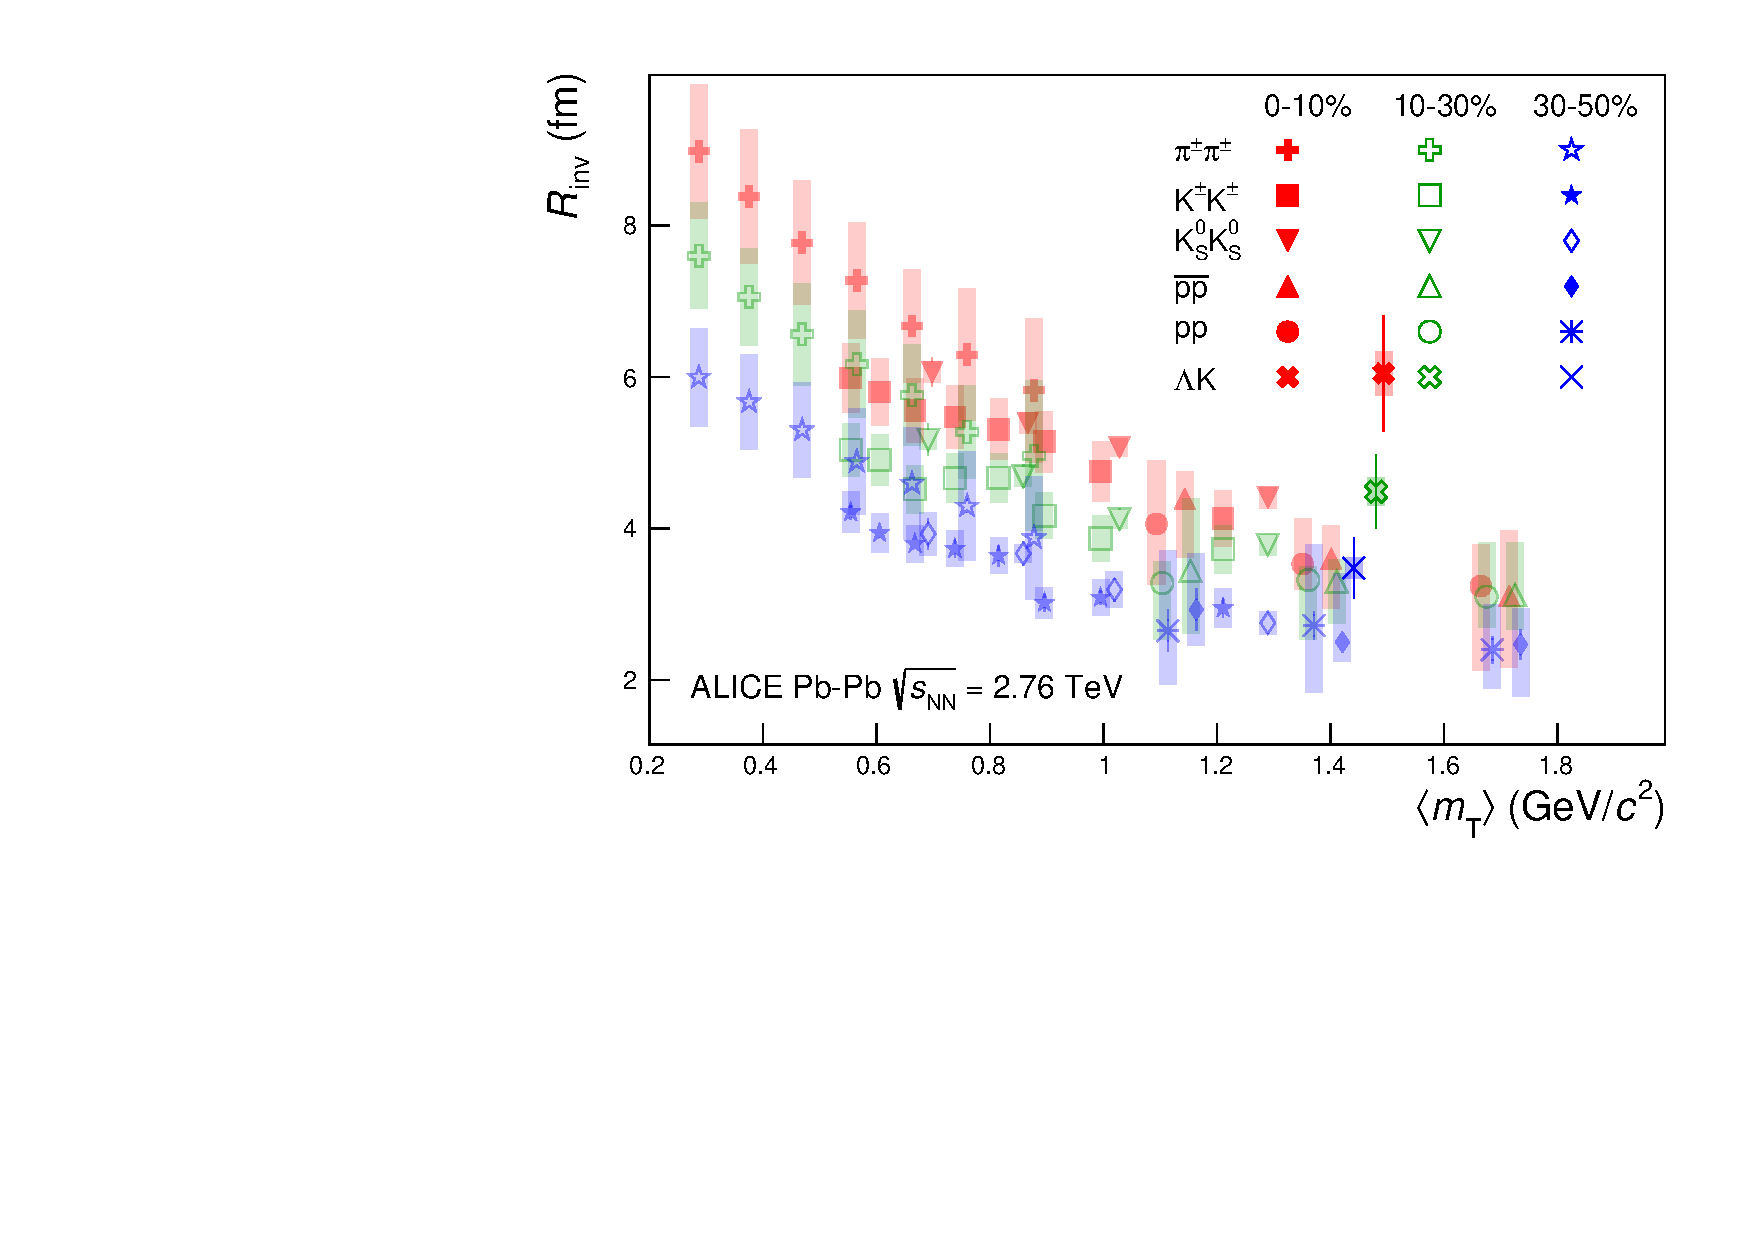
\includegraphics[width=0.75\textwidth]{\ResultsDirBaseLamKch\SaveNameModLamKch/Comparisons/mTscaling_MinvCalcv2_OthersTransparent_3Res_NoResStamp.pdf}
+  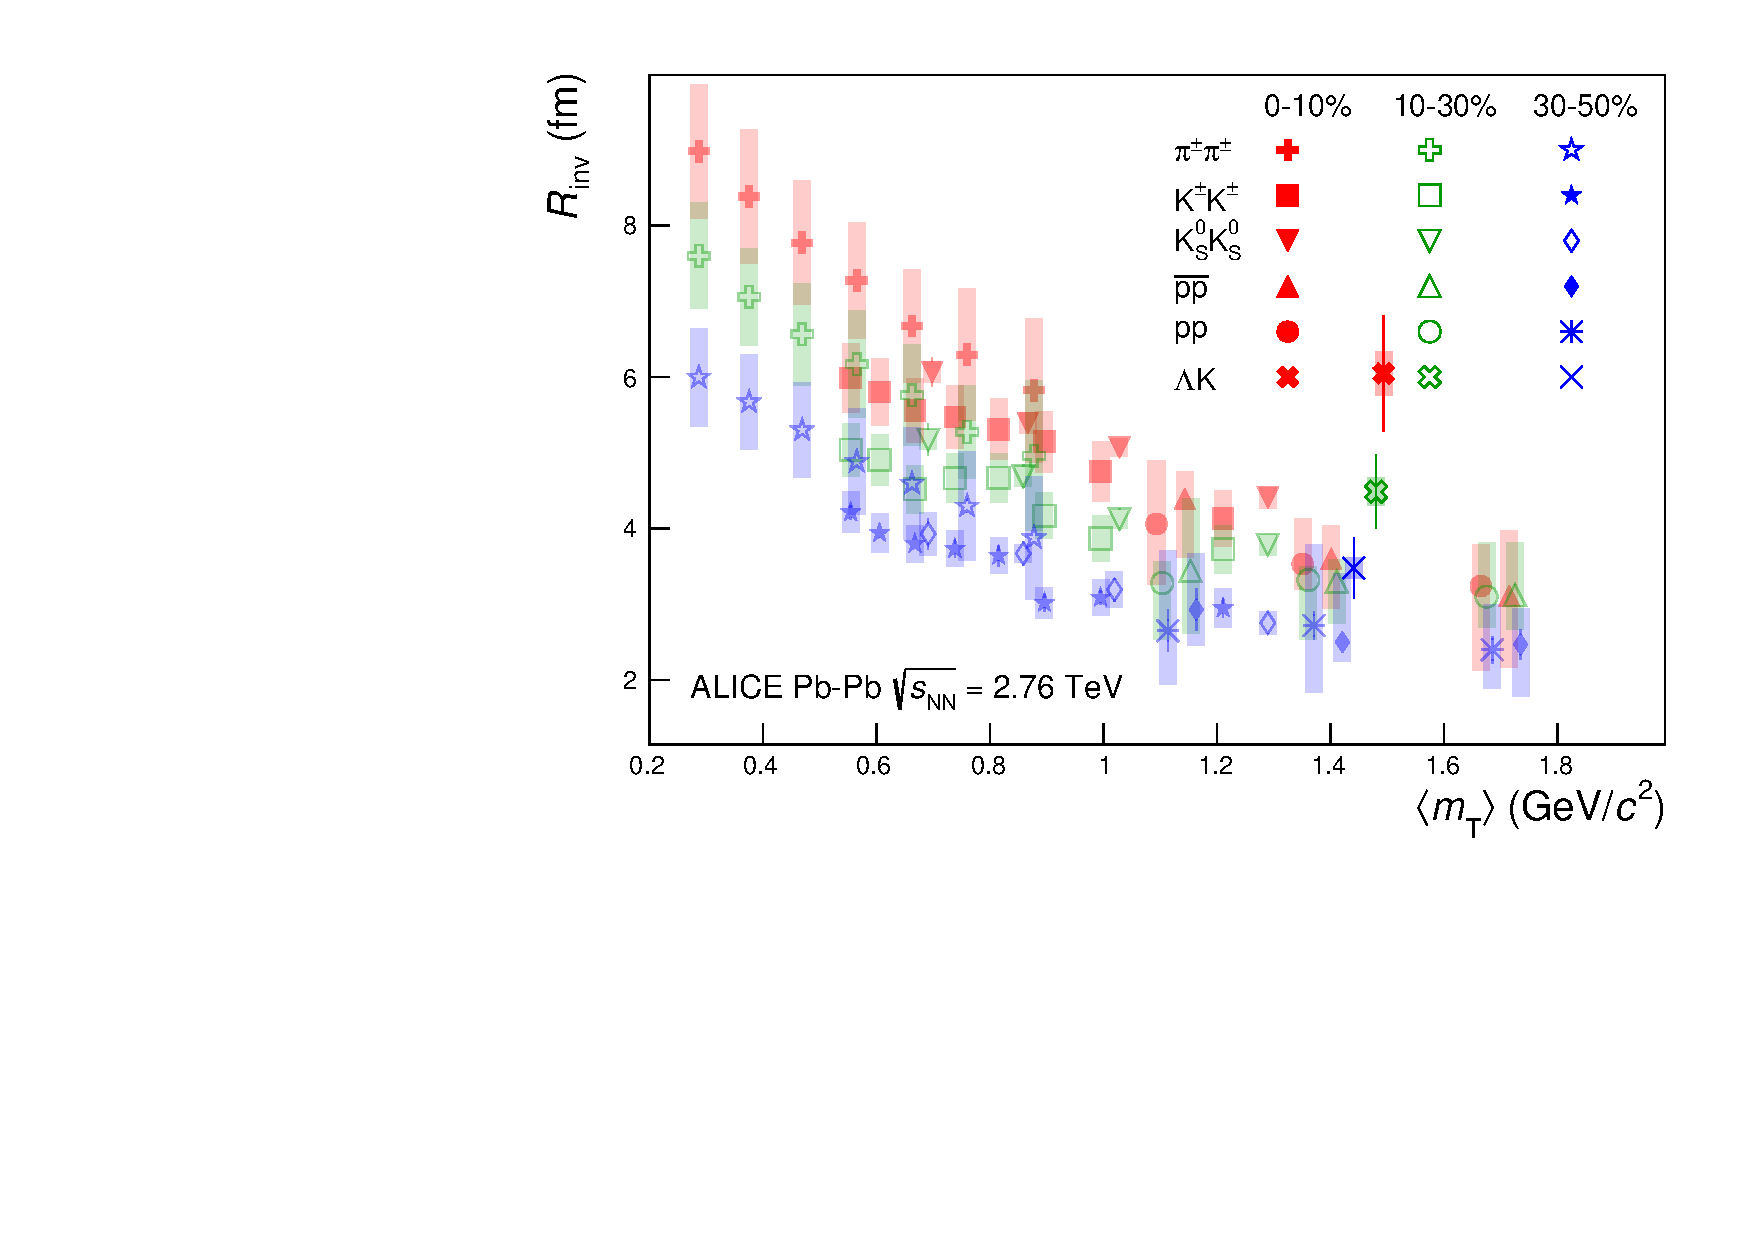
\includegraphics[width=0.60\textwidth]{\ResultsDirBaseLamKch\SaveNameModLamKch/Comparisons/mTscaling_MinvCalcv2_OthersTransparent_3Res_NoResStamp.pdf}
   \caption[\mt Scaling of Radii: 3 Residuals in Fit]
   {
   (Color online) Extracted fit $R_{\mathrm{inv}}$ parameters as a function of pair transverse mass (\mt) for several centralities.
-  Results from the \LamK analysis are presented together with ALICE published data \cite{Adam:2015vja} for various other pair systems.  
+  Results from the \LamK analysis are presented together with ALICE published data~\cite{Adam:2015vja} for various other pair systems.  
   }
   \label{fig:mTScalingOfRadii_3Res}
 \end{figure}
 
-Figure \ref{fig:ScattParams_3Res} (right) presents the $\lambda_{\mathrm{Fit}}$ vs. radius parameters for all three studied centrality bins.
+Figure~\ref{fig:ScattParams_3Res} (right) presents the $\lambda_{\mathrm{Fit}}$ and radius parameters for all three studied centrality percentile ranges.
 The $\lambda_{\mathrm{Fit}}$ parameters are expected to be close to unity. 
-A comparison of the extracted radii from this study to those of other systems measured by ALICE \cite{Adam:2015vja} is shown in Figure \ref{fig:mTScalingOfRadii_3Res}. 
-The figure shows extracted $R_{\mathrm{inv}}$ vs. \mt for several centralities and for several different pair systems.
-The \mt value used for the present \LamK results was taken as the average of the three systems\footnote[1]
-{
+A comparison of the extracted radii from this study to those of other systems measured by ALICE~\cite{Adam:2015vja} is shown in Fig.~\ref{fig:mTScalingOfRadii_3Res}. 
+The figure shows extracted $R_{\mathrm{inv}}$ as a function of \mt for several centrality ranges and for several different pair systems.
+The \mt value used for the present \LamK results was taken as the average of the three systems.
 For non-identical particle pairs, to be more directly analogous to the single particle \mt, the definition of the pair transverse mass used in this study is
-\begin{equation*}
+\begin{equation}
 \begin{aligned}
- m_{\mathrm{T, pair}}^{2} &= \left( \frac{m_{\mathrm{inv}}}{2} \right)^{2} + \left( \frac{1}{2} |\textbf{\textit{p}}_{\mathrm{T,1}} + \textbf{\textit{p}}_{\mathrm{T,2}}| \right)^{2} = (K^{0})^{2} - (K^{3})^{2} \quad \mathrm{where} ~~K^{\mu} \equiv \frac{1}{2} \left( p_{1}^{\mu} + p_{2}^{\mu} \right)
+ m_{\mathrm{T, pair}}^{2} &= \left( \frac{m_{\mathrm{inv}}}{2} \right)^{2} + \left( \frac{1}{2} |\textbf{\textit{p}}_{\mathrm{T,1}} + \textbf{\textit{p}}_{\mathrm{T,2}}| \right)^{2} = (K^{0})^{2} - (K^{3})^{2}, \quad \mathrm{where} ~~K^{\mu} \equiv \frac{1}{2} \left( p_{1}^{\mu} + p_{2}^{\mu} \right)
 \end{aligned}
 \label{eqn:PairmTv1}
-\end{equation*}
-}.
+\end{equation}
 The radii are observed to increase for more central events, as expected from a simple geometric picture of the collisions.
-For each pair system, the radii decrease with increasing \mt, as expected in the presence of collective radial flow \cite{Akkelin:1995gh}.
-It was found that \cite{Kisiel:2014upa}, even in the presence of good global \mt-scaling for the three-dimensional radii in the Longitudinally Co-Moving System (LCMS), a particle species dependence will exist for the $R_{\mathrm{inv}}$ measured in the PRF, due to trivial kinematic reasons.
-These kinematic effects, resulting from the transformation from LCMS to PRF, causes smaller masses to exhibit larger $R_{\mathrm{inv}}$ \cite{Adam:2015vja} (explaining, for instance, how the pion radii are systematically higher than kaon radii at the same approximate \mt).
-
-It is clear from the results in Fig.\ \ref{fig:mTScalingOfRadii_3Res} that the \LamK systems do not conform to the approximate \mt-scaling of the identical particle pair source sizes.
-When dealing with non-identical particles, the pair emission source is a superposition of two unique single-particle sources.
-The hydrodynamic nature of the medium produces the approximate \mt-scaling with respect to these single-particle sources, not the pair sources.
-For identical particle studies, in which the pair source is comprised of two identical single particle sources, the femtoscopic radii naturally follow the \mt-scaling trend.
-The hydrodynamic response of the system not only confines higher-\mt particles to smaller homogeneity regions, but also pushes their average emission points further in the ``out" direction \cite{Retiere:2003kf}.
-Therefore, the \Lam and K sources differ both in size and space-time location, with the \Lam source both smaller in size and further out in the fireball than that of the kaons.
-These effects can inflate the radii extracted using the one-dimensional Lednick\'y model, which assumes a spherically symmetric source with no offsets (i.e. $R_{\mathrm{out}} = R_{\mathrm{side}} = R_{\mathrm{long}}$ and $\mu_{\mathrm{out}} = \mu_{\mathrm{side}} = \mu_{\mathrm{long}} = 0$).
-This effect is demonstrated in Appendix \ref{App:THERM} using the THERMINATOR 2 simulation.
-The largest violation of the \mt-scaling is observed for the 0--10\% centrality bin, in which one expects the largest emission asymmetry.
-In summary, the large extracted \LamK radii support the hydrodynamic nature of the system dictating the femtoscopic substructure.
-
-The experimental data support the difference in mean emission space-time coordinates of the \Lam and K sources, called an ``emission asymmetry".
-In addition to the second moments of the pair distribution functions, non-identical particle studies are sensitive to the relative emission shifts, i.e. the first moments of the emission function \cite{Kisiel:2009eh}.
-A separation of the single-particle sources in the out direction is expected for \LamK pairs at mid-rapidity in Pb-Pb collisions.
+For each pair system, the radii decrease with increasing \mt, as expected in the presence of collective radial flow~\cite{Akkelin:1995gh}.
+It was found that~\cite{Kisiel:2014upa}, even in the presence of good global \mt-scaling for the three-dimensional radii in the Longitudinally Co-Moving System (LCMS), a particle species dependence will exist for the $R_{\mathrm{inv}}$ measured in the PRF, due to trivial kinematic reasons.
+These kinematic effects, resulting from the transformation from LCMS to PRF, causes smaller masses to exhibit larger $R_{\mathrm{inv}}$~\cite{Adam:2015vja} (explaining, for instance, how the pion radii are systematically higher than kaon radii at the same approximate \mt).
+
+It is clear from the results in Fig.~\ref{fig:mTScalingOfRadii_3Res} that the \LamK systems do not conform to the approximate \mt-scaling of the identical particle pair source sizes.
+The hydrodynamic nature of the medium produces the approximate \mt-scaling with respect to the single-particle sources, not the pair sources.
+Furthermore, the hydrodynamic response not only confines higher-\mt particles to smaller homogeneity regions, it also pushes their average emission points further in the ``out" direction~\cite{Retiere:2003kf}, in a coordinate system chosen according to the out-side-long prescription (where the ``long" axis is parallel to the beam, ``out" is parallel to the total transverse momentum of the pair, and ``side" is orthogonal to both).
+For identical particle studies, in which the pair source is comprised of two identical single particle sources commonly affected by the space-time shift, the femtoscopic radii naturally follow the \mt-scaling trend.
+However, for the case of non-identical particles, the pair emission source is a superposition of two unique single-particle sources, which are affected differently by the hydrodynamic response of the system.
+Therefore, the \Lam and K sources differ both in size and space--time location, leading to an ``emission asymmetry", with the \Lam source both smaller in size and further out in the fireball than that of the kaons.
+
+A separation of the single-particle sources in the ``out" direction is expected for \LamK pairs at mid-rapidity in Pb--Pb collisions, as described above, and the experimental data support such an emission asymmetry.
+In addition to the ``size" of the emitting region (more precisely, the second moments of the emission functions) accessible with identical particle studies, non-identical particle correlations are sensitive to the relative emission shifts, i.e., the first moments of the emission function~\cite{Kisiel:2009eh}.
 The spherical harmonic decomposition of the correlation function offers an elegant method for extracting information about the emission asymmetries.
 With this method, one can draw a wealth of information from just a few components of the decomposition.
-Particularly, the $C_{00}$ component is similar to the 1D correlation functions typically studied, and probes the overall size of the source.
-Of interest here, the $\Re C_{11}$ component probes the asymmetry of the system in the out direction; a non-zero value reveals the asymmetry. 
-Figure \ref{fig:LamKchP_ReC00C11_0010} shows the $C_{00}$ and $\Re C_{11}$ components from the spherical decomposition of the \LamKchP data in the 0--10\% centrality bin.
+Particularly, the $l=0$, $m=0$ component, $C_{00}$, is similar to the one-dimensional correlation functions typically studied, and probes the overall size of the source.
+Of interest here, the real part of the $l=1$, $m=1$ component, $\Re C_{11}$, probes the asymmetry of the system in the ``out" direction; a non-zero value reveals the asymmetry. 
+Figure~\ref{fig:LamKchP_ReC00C11_0010} shows the $C_{00}$ and $\Re C_{11}$ components from the spherical decomposition of the \LamKchP data in the 0--10\% centrality interval.
 The $\Re C_{11}$ component shows a clear deviation from zero, and the negative value signifies that the \Lam particles are, on average, emitted further out and/or earlier than the K mesons.
-This conclusion is supported by the results obtained from the THERMINATOR 2 model, shown in Fig.\ \ref{fig:LamKchP_StdThermSources}.
-Furthermore, as previously stated, a non-zero shift in the source will induce larger extracted radii within the Lednick\'y model, as demonstrated with the THERMINATOR 2 simulatin in App.\ \ref{App:THERM}.
+This conclusion is supported by the results obtained from the THERMINATOR 2 model, shown in Fig.~\ref{fig:LamKchP_StdThermSources}.
+Furthermore, this emission asymmetry effect can inflate the radii extracted with the one-dimensional Lednick\'y model, which assumes a spherically symmetric source with no offsets (i.e., $R_{\mathrm{out}} = R_{\mathrm{side}} = R_{\mathrm{long}}$ and $\mu_{\mathrm{out}} = \mu_{\mathrm{side}} = \mu_{\mathrm{long}} = 0$).
+This effect is demonstrated in Appendix~\ref{App:THERM} using the THERMINATOR 2 simulation.
+In Fig.~\ref{fig:mTScalingOfRadii_3Res}, the largest violation of the \mt-scaling for the \LamK system is observed for the 0--10\% centrality interval, in which one expects the largest emission asymmetry.
 
 \begin{figure}[h!]
   \centering
-  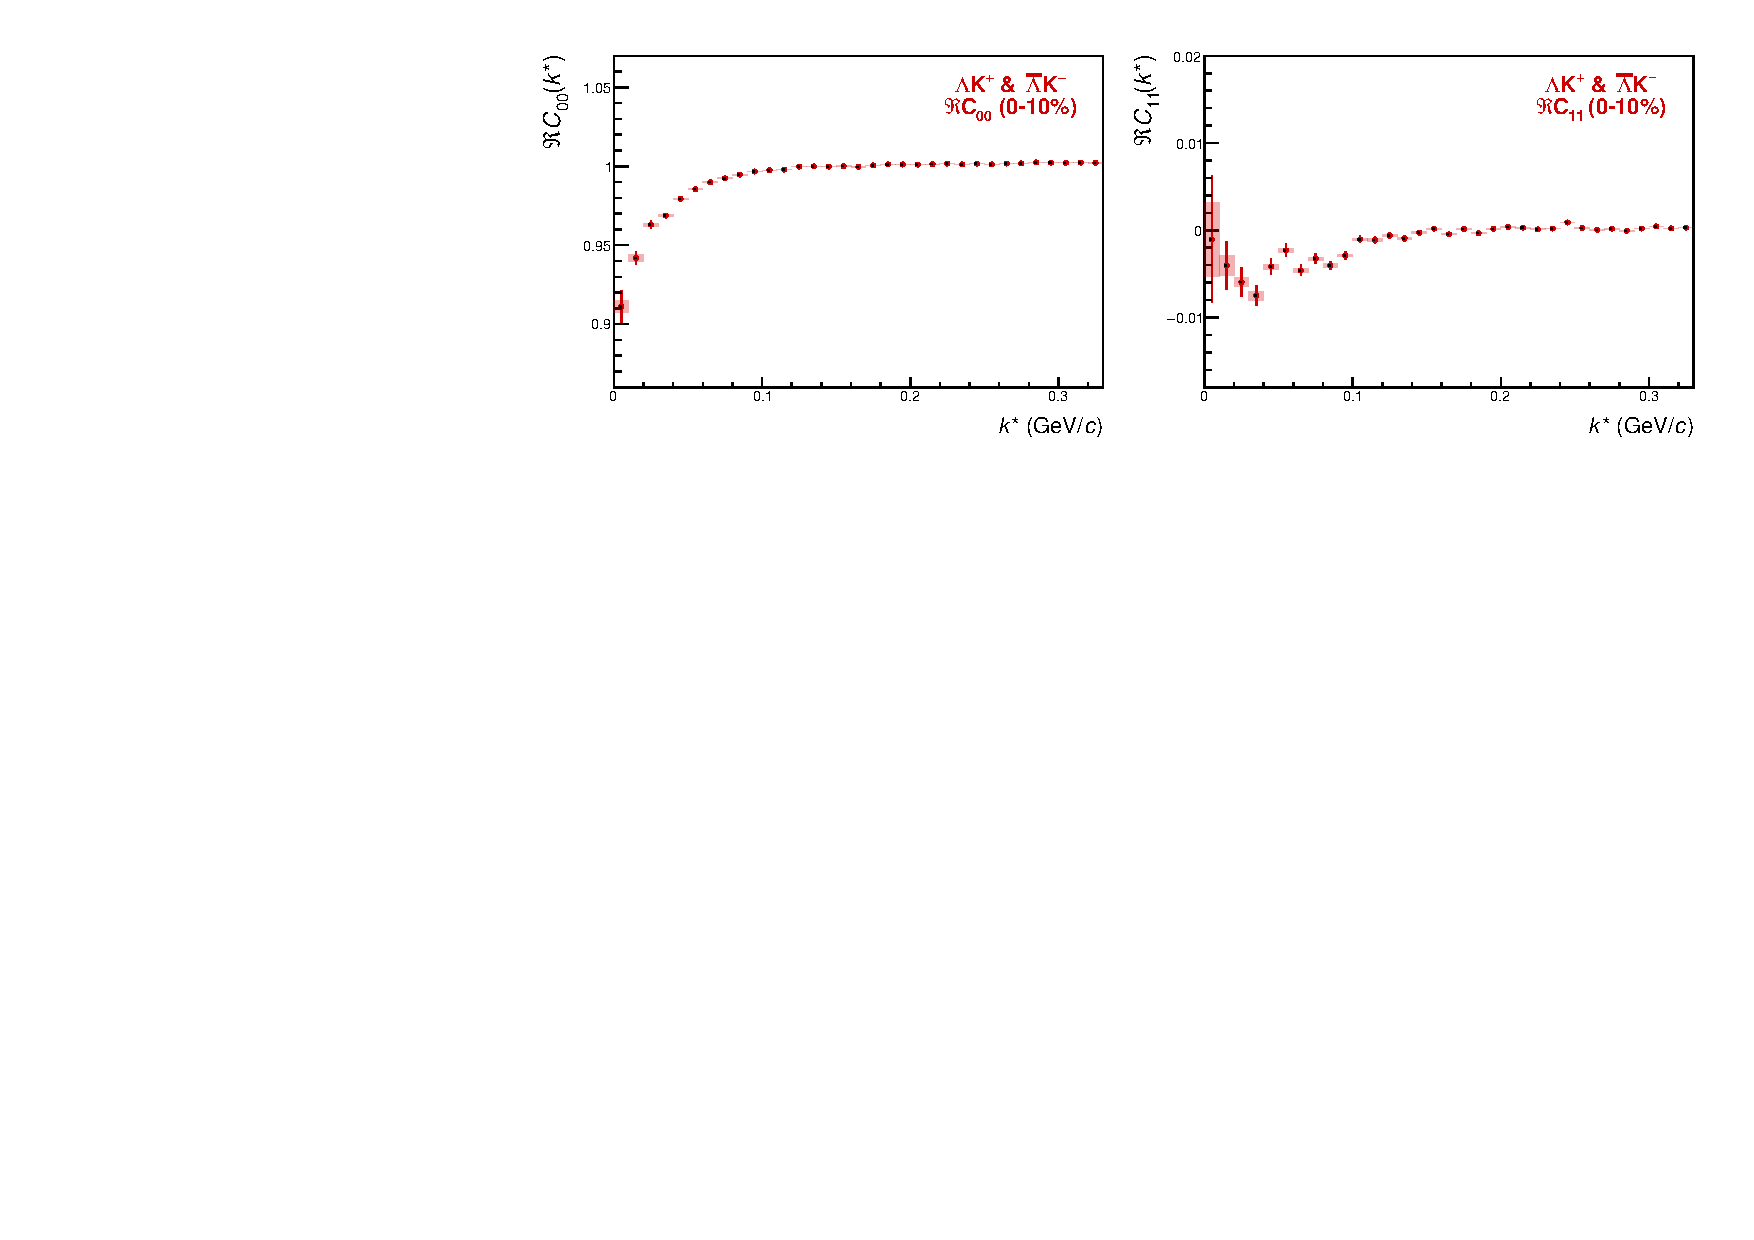
\includegraphics[width=0.8\textwidth]{\ResultsDirBase Results_cLamcKch_20181205/SphericalHarmonics/LamKchP/CanCfYlmReC00C11_LamKchPALamKchM_0010_wSysErr.pdf}
+  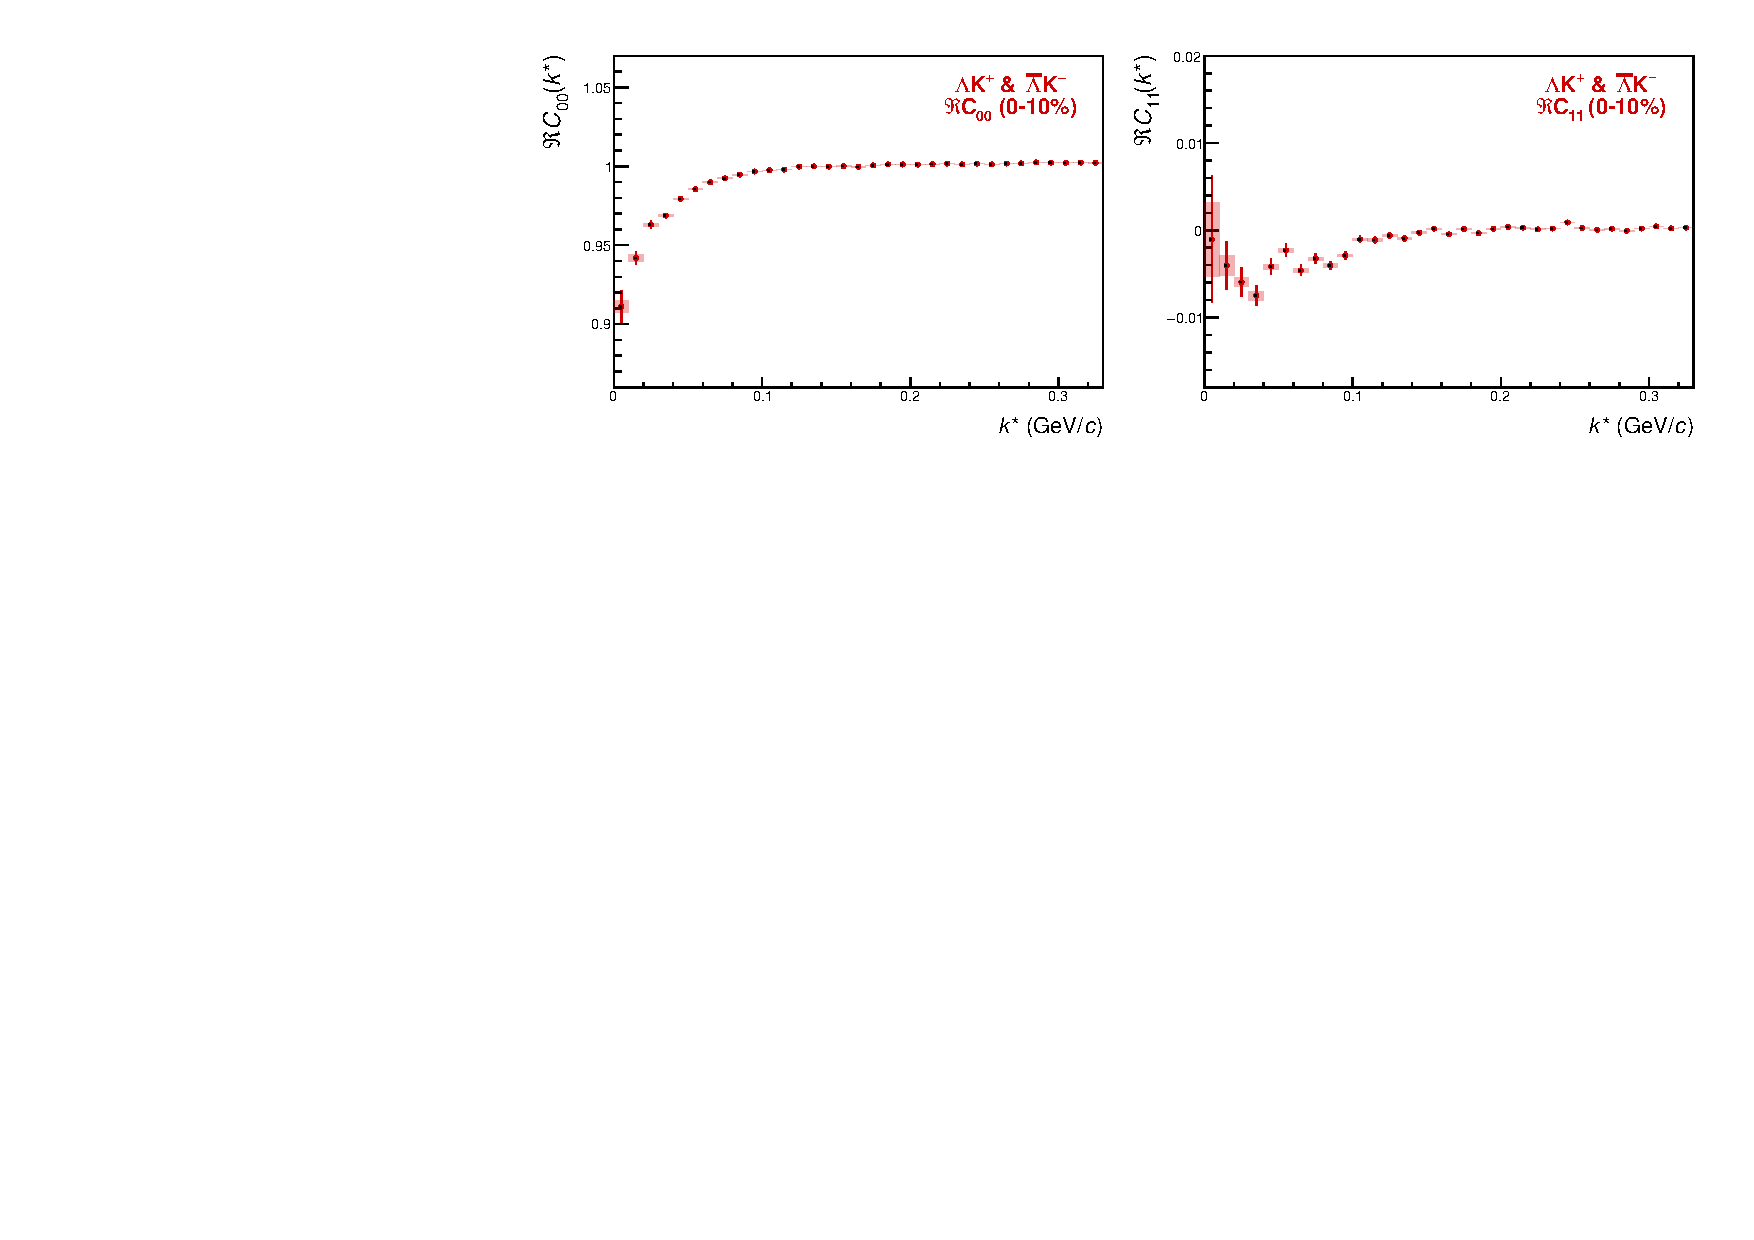
\includegraphics[width=\textwidth]{\ResultsDirBase Results_cLamcKch_20181205/SphericalHarmonics/LamKchP/CanCfYlmReC00C11_LamKchPALamKchM_0010_wSysErr.pdf}
   \caption[\LamKchP $C_{00}$ and $\Re C_{11}$ Spherical Harmonic Components (0--10\%)]
   {
-  (Color online) $C_{00}$ (left) and $\Re C_{11}$ (right) components of a spherical harmonic decomposition of the \LamKchP correlation function for the 0--10\% centrality bin.  
-The $C_{00}$ component is similar to the 1D correlation functions typically studied, and probes the overall size of the source.
-The $\Re C_{11}$ component probes the asymmetry in the system; a non-zero value reveals the asymmetry
+  (Color online) Spherical harmonics components $C_{00}$ (left) and $\Re C_{11}$ (right) of the \LamKchP correlation function for the 0--10\% centrality interval.  
+The $C_{00}$ component is similar to the one-dimensional correlation functions typically studied, and probes the overall size of the source.
+The $\Re C_{11}$ component probes the asymmetry in the system; a non-zero value reveals the asymmetry.
   }
   \label{fig:LamKchP_ReC00C11_0010}
 \end{figure}
@@ -983,15 +998,15 @@
 
 \subfile{\ResultsDirBaseLamKch\SaveNameModLamKch/Tables/ResultsTableTriple_Vert.tex}
 
-Results from a femtoscopic analysis of \LamK correlations in Pb-Pb collisions at $\sqrt{s_{\mathrm{NN}}}$ = 2.76 TeV with ALICE at the LHC have been presented, and are summarized in Table \ref{tab:FitResultsLamK_3Res}.
+Results from a femtoscopic analysis of \LamK correlations in Pb--Pb collisions at $\sqrt{s_{\mathrm{NN}}}$ = 2.76 TeV with ALICE at the LHC have been presented, and are summarized in Table~\ref{tab:FitResultsLamK_3Res}.
 The femtoscopic radii, $\lambda$ parameters, and scattering parameters were extracted from one-dimensional correlation functions in terms of the invariant momentum difference.
 The scattering parameters of \LamK pairs in all three charge combinations (\LamKchP, \LamKchM, and \LamKs) have been measured for the first time.
 Striking differences are observed in the \LamKchP, \LamKchM, and \LamKs correlation functions, which are reflected in the unique set of scattering parameters extracted for each.
 The extracted scattering parameters indicate that the strong force is repulsive in the \LamKchP interaction and attractive in the \LamKchM and \LamKs interactions.
-This effect could be due to different quark-antiquark interactions between the pairs, or from different net strangeness for each system. 
+This effect could be due to different quark--antiquark interactions between the pairs, or from different net strangeness for each system. 
 The non-femtoscopic background is found to result almost entirely from collective effects, and is described quantitatively with unprecedented precision with the THERMINATOR 2 event generator.
 Finally, the \LamK systems exhibit source radii larger than expected from extrapolation from identical particle femtoscopic studies.
-This effect is interpreted as resulting from the separation in space-time of the single-particle \Lam and K source distributions.
+This effect is interpreted as resulting from the separation in space--time of the single-particle \Lam and K source distributions (i.e., the emission asymmetry of the source).
 %\clearpage
 
 %%%%% acknowledgements
@@ -1020,27 +1035,27 @@
 
 %************************************************************************************************************************
 %************************************************************************************************************************
-\section{Stavinskiy Reference Method}
+\section{Stavinskiy reference method}
 \label{App:StavMethod}
 
-Another option for obtaining the reference distribution, $B(k^{*})$, is to use, what will be referred to as, the ``Stavinskiy method" \cite{Stavinskiy04}.
-The method was first proposed to handle the case of one event femtoscopy, and has been suggested for use in eliminating momentum conservation effects in the reference distribution \cite{Lisa:2005dd}.
+Another option for obtaining the reference distribution, $B(k^{*})$, is to use, what will be referred to as, the ``Stavinskiy method"~\cite{Stavinskiy04}.
+The method was first proposed to handle the case of one event femtoscopy, and has been suggested for use in eliminating momentum conservation effects in the reference distribution~\cite{Lisa:2005dd}.
 The method is appropriate for collisions between symmetric projectiles, at sufficiently large energy, with a detector which is symmetrical with respect to the transition $\mathbf{r} \rightarrow \mathbf{-r}$.
-The use of this method in a three-dimensional analysis of two-pion correlations produced, in comparison to the event mixing results, an increase of 6\% for $R_{\mathrm{side}}$ at low-$k_{\mathrm{T}}$ and up to 4\% for $R_{\mathrm{out}}$ and $R_{\mathrm{long}}$ \cite{Aamodt:2011mr}.
+The use of this method in a three-dimensional analysis of two-pion correlations produced, in comparison to the event mixing results, an increase of 6\% for $R_{\mathrm{side}}$ at low-$k_{\mathrm{T}}$ and up to 4\% for $R_{\mathrm{out}}$ and $R_{\mathrm{long}}$~\cite{Aamodt:2011mr}.
 The purpose of using the Stavinskiy method in this \LamK analysis is to rid the correlation functions of the non-femtoscopic background.  
 More specifically, the intent is to handle background contributions from elliptic flow, and other sources having reflection symmetry in the transverse plane.  
 With the Stavinskiy method, mixed-event pairs are not used for the reference distribution; instead, same-event pseudo-pairs, formed by rotating one particle in a real pair by 180$^\circ$ in the transverse plane, are used.  
 This rotation rids the pairs of any femtoscopic correlation, while maintaining correlations due to elliptic flow (and other suitably symmetric contributors).
-Care needs to be taken in treating the pseudo-pairs exactly like the real pairs; e.g. the pseudo-pairs should be exposed to the same pair cuts used in the analysis on the real pairs.
-The results of correctly implementing such a procedure are shown in Figure \ref{fig:StavCfs_Correct_LamKchP}.  
-The figure shows the Stavinskiy method does a very good job of ridding the \LamKchP correlations of their non-femtoscopic backgrounds.  
+Care needs to be taken in treating the pseudo-pairs exactly like the real pairs; e.g., the pseudo-pairs should be exposed to the same pair cuts used in the analysis on the real pairs.
+The results of correctly implementing such a procedure are shown in Fig.~\ref{fig:StavCfs_Correct_LamKchP}.
+The figure demonstrates, for the \LamKchP system, that the Stavinskiy method is effective in flattening the correlation function in the region where no femtoscopic signal is expected.
 
 \begin{figure}[h!]
   \centering
   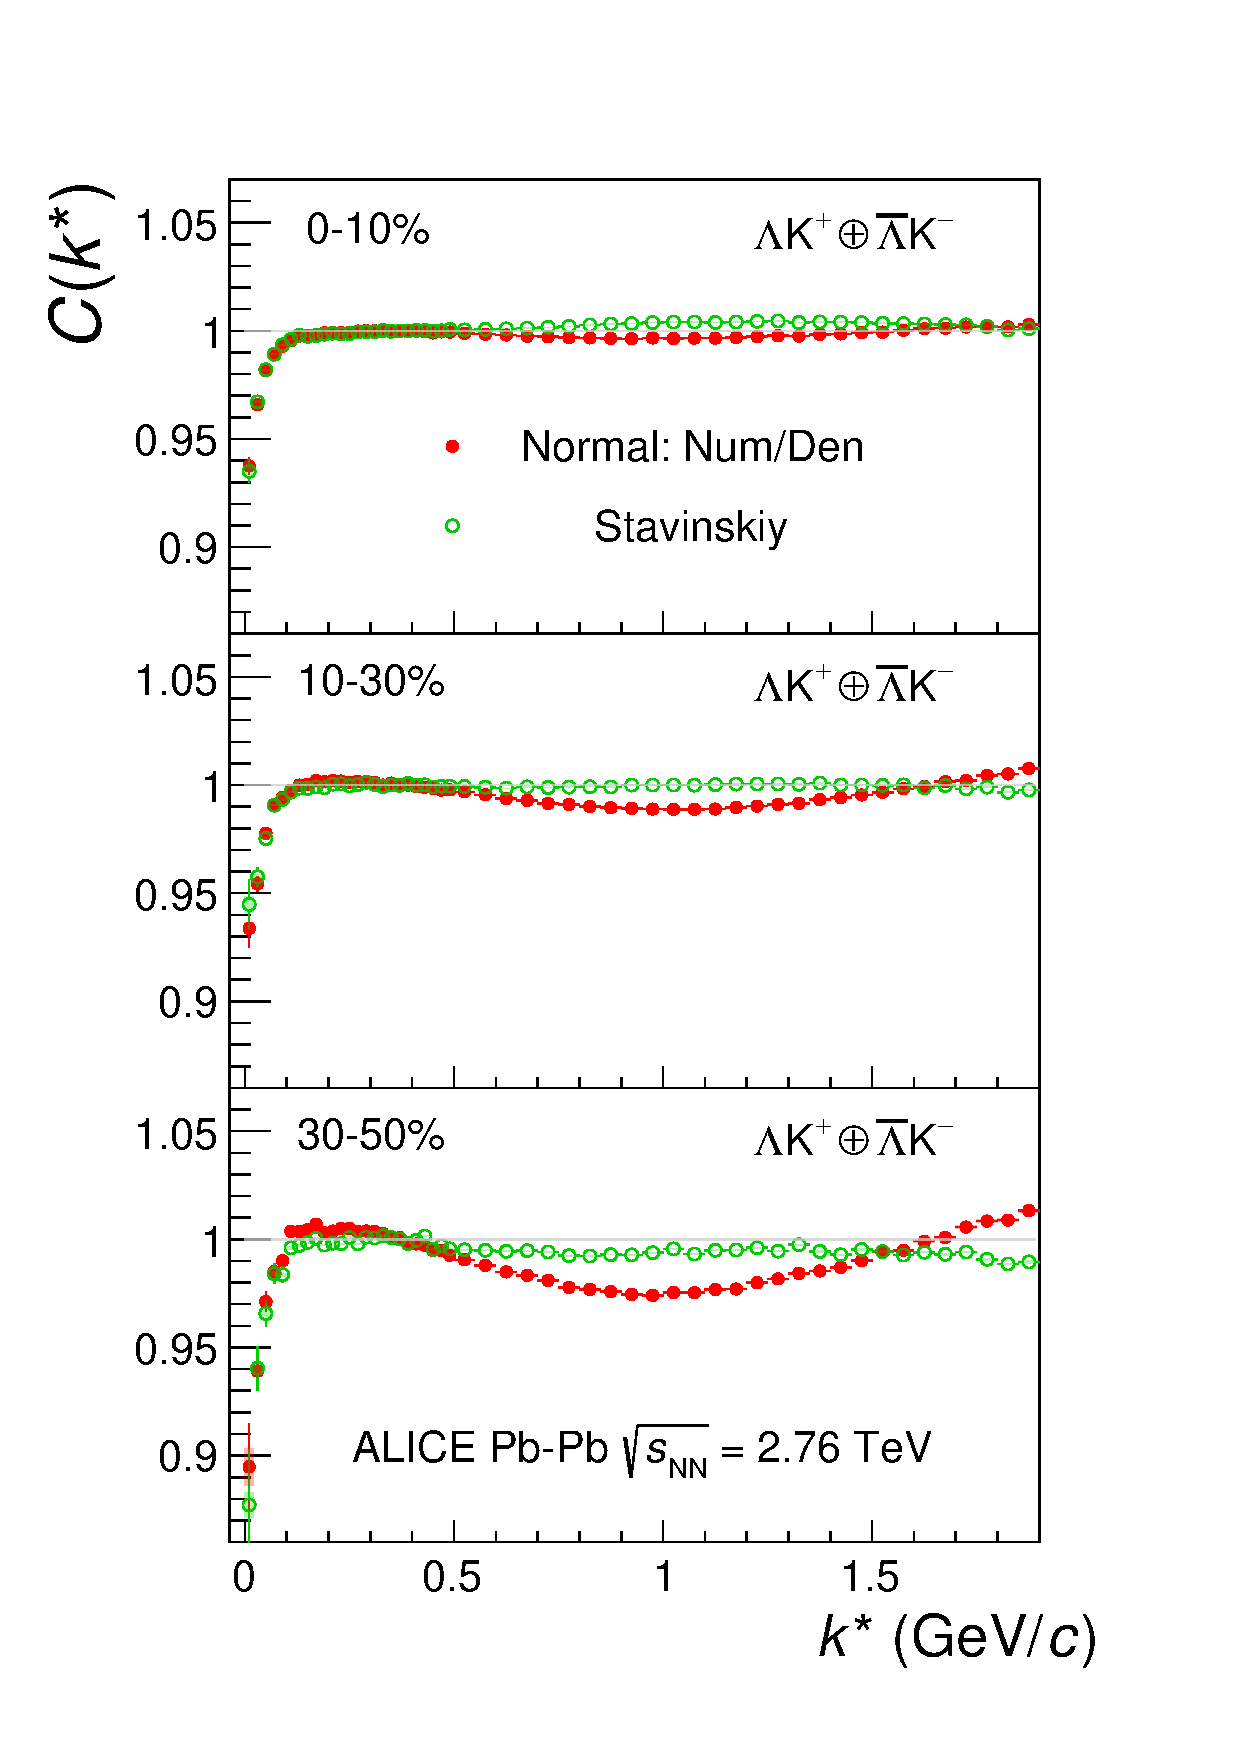
\includegraphics[width=0.667\textwidth]{/home/jesse/Analysis/FemtoAnalysis/AnalysisNotes/4_CorrelationFunctions/Figures/OnlyTwo/canKStarCfsLamKchPCombConj_20190319vs20190319StavCf_CustomRebin.pdf}
   \caption[\LamKchP Stavinskiy Correlation Functions]
   {
-  (Color online) \LamKchPALamKchM correlation functions built using the Stavinskiy method for 0--10\%, 10--30\%, and 30--50\% centralities.  Closed symbols represent correlations built using the normal mixed-event reference distribution, while open symbols represent correlations formed using the Stavinskiy same-event pseudo-pairs as a reference.
+  (Color online) Correlation functions for the $\Lambda\mathrm{K^{+}}\oplus\overline{\Lambda}\mathrm{K^{-}}$ system built using the Stavinskiy method for 0--10\%, 10--30\%, and 30--50\% centrality intervals.  Closed symbols represent correlations built using the normal mixed-event reference distribution, while open symbols represent correlations formed using the Stavinskiy same-event pseudo-pairs as a reference.
   }
   \label{fig:StavCfs_Correct_LamKchP}
 \end{figure} 
@@ -1049,49 +1064,48 @@
 
 %************************************************************************************************************************
 %************************************************************************************************************************
-\section{Strong and Coulomb Fitter}
+\section{Strong and Coulomb fitter}
 \label{App:CoulombFitter}
 
-When modeling systems which include both strong and Coulomb effects, Eq.\ \ref{eqn:LednickyEqn} is no longer valid, and, in fact, there is no analytical form with which to fit.
-To solve such a problem, and to fit such a system, one must develop a more fundamental model, beginning with Eq.\ \ref{eqn:KooninPrattEqn} and using the two-particle wave-function including both strong and Coulomb interactions \cite{Lednicky:2005tb}:
-
-\begin{equation}
- \Psi_{\mathbf{k^{*}}}(\mathbf{r^{*}}) = e^{i\delta_{c}}\sqrt{A_{c}(\eta)}[e^{i\mathbf{k^{*}} \cdot \mathbf{r^{*}}}F(-i\eta,1,i\xi) + f_{c}(k^{*})\frac{\tilde{G}(\rho,\eta)}{r^{*}}]
+When modeling systems which include both strong and Coulomb effects, Eq.~\ref{eqn:LednickyEqn} is no longer valid, and there exists no analytical form with which to fit.
+To model such a system, a more fundamental approach must be taken, beginning with Eq.~\ref{eqn:KooninPrattEqn} and using the two-particle wave-function which includes both strong and Coulomb interactions~\cite{Lednicky:2005tb},
+\begin{equation}
+ \Psi_{\mathbf{k^{*}}}(\mathbf{r^{*}}) = e^{i\delta_{\mathrm{c}}}\sqrt{A_{\mathrm{c}}(\eta)}[e^{i\mathbf{k^{*}} \cdot \mathbf{r^{*}}}F(-i\eta,1,i\xi) + f_{\mathrm{c}}(k^{*})\frac{\tilde{G}(\rho,\eta)}{r^{*}}],
 \label{eqn:CoulombWaveFcn}
 \end{equation}
-
-where $\rho = k^{*}r^{*}$, $\eta = (k^{*}a_{c})^{-1}$, $\xi = \mathbf{k^{*}} \cdot \mathbf{r^{*}} + k^{*}r^{*} \equiv \rho(1+\cos\theta^{*})$, and $a_{c} = (\mu z_{1}z_{2}e^{2})^{-1}$ is the two-particle Bohr radius (including the sign of the interaction).  
-$\delta_{c}$ is the Coulomb s-wave phase shift, $A_{c}(\eta)$ is the Coulomb penetration factor, $\tilde{G} = \sqrt{A_{c}}(G_{0} + iF_{0})$ is a combination of the regular ($F_{0}$) and singular ($G_{0}$) s-wave Coulomb functions.  
-$f_{c}(k^{*})$ is the s-wave scattering amplitude
-\begin{equation}
- f_{c}(k^{*}) = \left[\frac{1}{f_{0}} + \frac{1}{2}d_{0}k^{*2} - \frac{2}{a_{c}}h(\eta) - ik^{*}A_{c}(\eta)\right]^{-1}
+where $\rho = k^{*}r^{*}$, $\eta = (k^{*}a_{\mathrm{c}})^{-1}$, $\xi = \mathbf{k^{*}} \cdot \mathbf{r^{*}} + k^{*}r^{*} \equiv \rho(1+\cos\theta^{*})$, and $a_{\mathrm{c}} = (\mu z_{1}z_{2}e^{2})^{-1}$ is the two-particle Bohr radius (including the sign of the interaction).  
+Furthermore, $\delta_{\mathrm{c}}$ is the Coulomb s-wave phase shift, $A_{\mathrm{c}}(\eta)$ is the Coulomb penetration factor, $\tilde{G} = \sqrt{A_{c}}(G_{0} + iF_{0})$ is a combination of the regular ($F_{0}$) and singular ($G_{0}$) s-wave Coulomb functions.  
+Finally, $f_{\mathrm{c}}(k^{*})$ is the s-wave scattering amplitude,
+\begin{equation}
+ f_{\mathrm{c}}(k^{*}) = \left[\frac{1}{f_{0}} + \frac{1}{2}d_{0}k^{*2} - \frac{2}{a_{\mathrm{c}}}h(\eta) - ik^{*}A_{\mathrm{c}}(\eta)\right]^{-1},
 \label{eqn:CoulombScattAmp}
 \end{equation}
-where, the ``h-function", $h(\eta$), is expressed through the digamma function, $\psi(z)$ = $\Gamma'(z)/\Gamma(z)$ as
-\begin{equation}
- h(\eta) = 0.5[\psi(i\eta) + \psi(-i\eta) - \ln(\eta^{2})]
+where the ``h-function", $h(\eta$), is expressed through the digamma function, $\psi(z)$ = $\Gamma'(z)/\Gamma(z)$ as
+\begin{equation}
+ h(\eta) = 0.5[\psi(i\eta) + \psi(-i\eta) - \ln(\eta^{2})].
 \label{eqn:LednickyHFunction}
 \end{equation} 
-In this case, the $\lambda$ parameter may be included as: 
-\begin{equation}
- C(\mathbf{k^{*}}) = (1 - \lambda) + \lambda\int S(\mathbf{r^{*}})|\Psi^{S}_{\mathbf{k^{*}}}(\mathbf{r^{*}})|^{2}d^{3}\mathbf{r^{*}}
+In this case, the $\lambda$ parameter may be included as
+\begin{equation}
+ C(\mathbf{k^{*}}) = (1 - \lambda) + \lambda\int S(\mathbf{r^{*}})|\Psi^{S}_{\mathbf{k^{*}}}(\mathbf{r^{*}})|^{2}d^{3}\mathbf{r^{*}}.
 \label{eqn:GenCfEqnwLambda}
 \end{equation}
 To build a fit function for a system including both strong and Coulomb interactions two related options were considered. 
-The first option was to numerically integrate Eq.\ \ref{eqn:KooninPrattEqn}.  
-The second option was to simulate a large sample of particle pairs, calculate the wave function describing the interaction, and average to obtain the integral in Eq.\ \ref{eqn:KooninPrattEqn}. 
-
-
-%************************************************************************************************************************
-%************************************************************************************************************************
-\section{Relative Emission Shifts with THERMINATOR 2}
+The first option was to numerically integrate Eq.~\ref{eqn:KooninPrattEqn}.  
+The second option was to simulate a large sample of particle pairs, calculate the wave function describing the interaction, and average to obtain the integral in Eq.~\ref{eqn:KooninPrattEqn}. 
+For this analysis, the latter option was adopted.
+
+
+%************************************************************************************************************************
+%************************************************************************************************************************
+\section{Relative emission shifts with THERMINATOR 2}
 \label{App:THERM}
 
-Fig.\ \ref{fig:LamKchP_StdThermSources} shows \LamKchP results from the THERMINATOR 2 event generator for an impact parameter of $b = 2$ fm.
+Figure~\ref{fig:LamKchP_StdThermSources} shows \LamKchP results from the THERMINATOR 2 event generator for an impact parameter of $b = 2$ fm.
 As THERMINATOR 2 does not include any final state effects, the femtoscopic correlation was introduced by assuming a set of scattering parameters ($\Re f_{0},\, \Im f_{0},\, d_{0}$) = ($-$0.60 fm, 0.51 fm, 0.83 fm) and weighting the signal distribution (numerator pairs) with the modulus squared of the two-particle wave function, $|\Psi|^{2}$.
 
-The top row of Fig. \ref{fig:LamKchP_StdThermSources} shows the experimental $\Lambda\mathrm{K}^{+}\oplus\overline{\Lambda}\mathrm{K}^{-}$ data together with the simulation results for the one-dimension correlation function (top left) and for the $\Re C_{11}$ component of the spherical harmonic decomposition (top right).
-The other four plots in Fig.\ \ref{fig:LamKchP_StdThermSources} show the source distribution from the simulation in the out (middle left), side (middle right), and long (bottom left) directions, as well as the temporal characteristics of the source (bottom right), all measured in the PRF.
+The top row of Fig.~\ref{fig:LamKchP_StdThermSources} shows the experimental $\Lambda\mathrm{K}^{+}\oplus\overline{\Lambda}\mathrm{K}^{-}$ data together with the simulation results (a) for the one-dimensional correlation function and (b) for the real part of the $l=1$, $m=1$ component, $\Re C_{11}$, of the spherical harmonic decomposition.
+The other four plots in Fig.~\ref{fig:LamKchP_StdThermSources} show the two-particle emission function (i.e., the pair separation distributions) from the simulation in the (c) out ($r^{*}_{\mathrm{out}}$), (d) side ($r^{*}_{\mathrm{side}}$), and (e) long ($r^{*}_{\mathrm{long}}$) directions, as well as (f) the temporal characteristics of the source ($\Delta t^{*}$), all measured in the PRF.
 The source distributions have all been fitted with a Gaussian form, the results of which are printed within the respective plots.
 One immediately sees a significant spatial shift in the out direction, $\mu_{\mathrm{out}} \approx$ 4 fm, and negligible shift in the other two directions, $\mu_{\mathrm{side}} \approx \mu_{\mathrm{long}} \approx$ 0 fm.
 In other words, the figure demonstrates that, within the THERMINATOR 2 model, the \Lam is, on average, emitted further out than its K partner.
@@ -1104,9 +1118,9 @@
   \caption[THERMINATOR 2 simulatin for \LamKchP]
   {
   Results from the THERMINATOR 2 simulation implemented with an impact parameter $b = 2$ fm for the \LamKchP pair system.
-  (Top left) the one-dimensional correlation function from THERMINATOR 2 together with the experimental data.
-  (Top right) the $\Re C_{11}$ component of a spherical harmonic decomposition of the THERMINATOR 2 simulation together with the experimental data.
-  The other four panels show the source distribution from the simulation in the out (middle left), side (middle right), and long (bottom left) directions, as well as the temporal characteristics (bottom right), all in the PRF.
+  (a) the one-dimensional correlation function from THERMINATOR 2 together with the experimental data.
+  (b) the $\Re C_{11}$ component of a spherical harmonic decomposition of the THERMINATOR 2 simulation together with the experimental data.
+  The other four panels show the source distribution from the simulation in the (c) out, (d) side, and (e) long directions, as well as (f) the temporal characteristics, all in the PRF.
   The source distributions have all been fitted with a Gaussian form, the results of which are printed within the respective plots.
   }
   \label{fig:LamKchP_StdThermSources}
@@ -1120,15 +1134,12 @@
 In all, $R_{\mathrm{out}} = R_{\mathrm{side}} = R_{\mathrm{long}}$ = 5 fm, and $\mu_{\mathrm{side}} = \mu_{\mathrm{long}}$ = 0 fm.
 The cases of $\mu_{\mathrm{out}}$ = 0 fm, $\mu_{\mathrm{out}}$ = 1 fm, $\mu_{\mathrm{out}}$ = 3 fm, and $\mu_{\mathrm{out}}$ = 6 fm were studied within the simulation.
 Note, within this implementation there is no time difference in the emission of the \Lam and K particles.
-For each, a one-dimensional correlation function is generated and fit with the Lednick\'y model, as shown in Fig.\ \ref{fig:LamKchP_ThermSources_VaryMuOut}).
+For each, a one-dimensional correlation function is generated and fit with the Lednick\'y model, as shown in Fig.~\ref{fig:LamKchP_ThermSources_VaryMuOut}.
 The scattering parameters are known precisely here, as they served as the weights used in the simulation, and are kept constant in the fit.
 Only the extracted one-dimensional source size is of interest here, so the $\lambda$ parameter is also fixed at unity.
 The figure demonstrates that as the separation $\mu_{\mathrm{out}}$ increases, so do the extracted femtoscopic radii.
-Figure \ref{fig:LamKchP_ThermSources_VaryMuOut_SH} shows, together with the experimental \LamKchP data, the effect of increasing $\mu_{\mathrm{out}}$ on the $\Re C_{00}$ and $\Re C_{11}$ components of the spherical harmonic decomposition.
+Figure~\ref{fig:LamKchP_ThermSources_VaryMuOut_SH} shows, together with the experimental \LamKchP data, the effect of increasing $\mu_{\mathrm{out}}$ on the spherical harmonic $l=0$, $m=0$ component, $C_{00}$, and on the real part of the $l=1$, $m=1$ component, $\Re C_{11}$.
 The figures shows that as $\mu_{\mathrm{out}}$ increases, so does the magnitude of the $\Re C_{11}$ signal.
-
-
-
 
 
 \begin{figure}[h]
@@ -1153,7 +1164,7 @@
   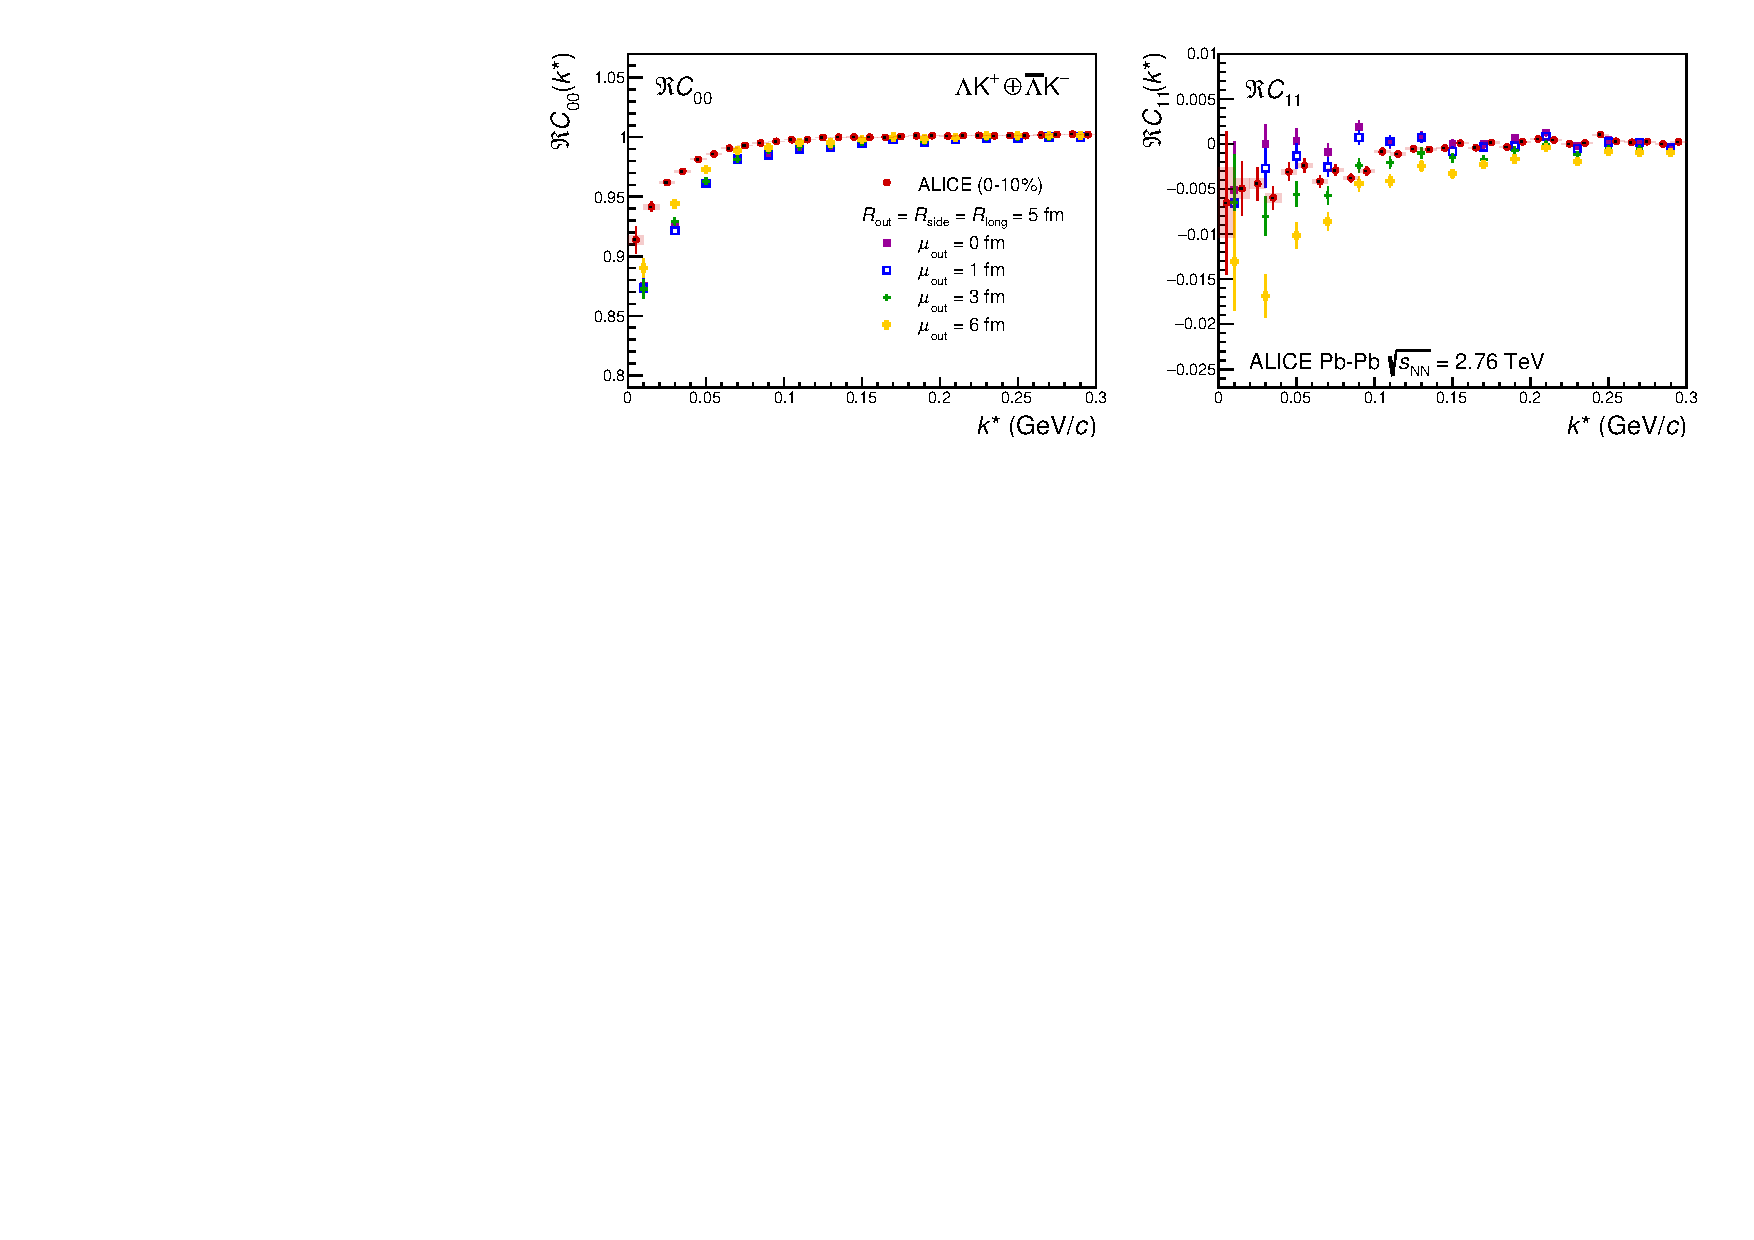
\includegraphics[width=\textwidth]{/home/jesse/Analysis/FemtoAnalysis/AnalysisNotes/7_ResultsAndDiscussion/7.1_ResultsLamK/7.1.2_ResultsLamK_DiscussionOfmTScaling/ThermPlots/LamKchP/CanCompFourThermCfYlmReC00C11_Full_RandomEPs_LamKchPALamKchM.pdf}
   \caption[\LamKchP $C_{00}$ and $\Re C_{11}$ Spherical Harmonic Components (0--10\%) with THERMINATOR 2 ($b = 2$ fm]
   {
-  (Color online) $C_{00}$ (left) and $\Re C_{11}$ (right) components of a spherical harmonic decomposition of the \LamKchP correlation function for the 0--10\% centrality bin shown with results from the THERMINATOR 2 simulation implemented with different shifts in the outward direction, $\mu_{\mathrm{out}}$, as described in the text.
+  (Color online) Spherical harmonics components $C_{00}$ (left) and $\Re C_{11}$ (right) of the \LamKchP correlation function for the 0--10\% centrality interval shown with results from the THERMINATOR 2 simulation implemented with different shifts in the outward direction, $\mu_{\mathrm{out}}$, as described in the text.
   }
   \label{fig:LamKchP_ThermSources_VaryMuOut_SH}
 \end{figure}

